%%%%%%%%%%%%%%%%%%%%%%%%%%%%%%%%%%%%%%%%%
% DSLSC Final Essay — Chicago Ridesourcing
%%%%%%%%%%%%%%%%%%%%%%%%%%%%%%%%%%%%%%%%%

\documentclass[10pt, a4paper]{article}
\usepackage[a4paper,left=2cm,right=2cm,top=2.5cm,bottom=2.5cm]{geometry}
\usepackage[english]{babel}
\usepackage[utf8x]{inputenc}
\usepackage{amsmath}
\usepackage{graphicx}
\usepackage{multirow}
\usepackage[colorinlistoftodos]{todonotes}

\setcounter{tocdepth}{3}

\begin{document}

\begin{titlepage}
\newcommand{\HRule}{\rule{\linewidth}{0.5mm}}
\center
\textsc{\LARGE Universit\`a degli Studi di Milano-Bicocca}\\[1cm]
\textsc{\Large Data Science Lab for Smart Cities}\\[0.3cm]
\textsc{\large Final Essay}\\[0.1cm]
\HRule \\[0.4cm]
{ \huge \bfseries Ridesourcing and Mobility Equity in Chicago}\\[0.4cm]
\HRule \\[1.5cm]
\large
\emph{Authors:}\\
Francesca Negri - 809625 - f.negri17@campus.unimib.it \\
Silvia Forcina Barrero - 819130 - s.forcinabarrero@campus.unimib.it \\[1cm]
{\large \today}\\[2cm]

\includegraphics{figs/logo.png}\\[1cm]
\vfill
\end{titlepage}

\begin{abstract}
Does ridesourcing in Chicago act as a mobility equaliser in transit-poor, vulnerable peripheries, or as a costly substitute where public transport is already strong? We analyse 75 Community Areas in 2024 (O'Hare excluded) using the Transport Usage Index (TUI), composite vulnerability scores, a Transit Accessibility Index built from CTA infrastructure and GTFS weekday departures, income-normalised Weighted TUI, and mean ridesourcing travel time to the Loop.

TUI peaks in central and lakefront areas and correlates negatively with vulnerability (Pearson $r$ up to $-0.54$, $p<0.001$) and positively with transit access ($r=0.75$). Spatial clustering is pronounced (Moran's $I=0.61$, $p=0.001$). A Spatial Error Model on $\log(1+\mathrm{TUI})$ is preferred over a spatial lag specification (AIC 75.2 vs.\ 80.0). The compensatory hypothesis is rejected: ridesourcing reinforces urban cores rather than filling public transport gaps in peripheral communities.
\end{abstract}

\renewcommand{\contentsname}{Summary}
\tableofcontents
\newpage

\section{Problem Description and Indicators}

\subsection{Introduction}
    Smart-city mobility policy increasingly treats digital platforms as part of urban transport infrastructure alongside buses, rail, and cycling networks. Real-time matching, cashless payment, and citywide coverage make Transportation Network Providers (TNP) such as Uber and Lyft attractive to planners seeking flexible capacity. Yet their private, fare-based model differs fundamentally from public transit: access depends on willingness and ability to pay, and trip records rarely identify where passengers live. Equity analysis must therefore ask not only where platforms operate, but who bears the cost relative to local income and how usage relates to existing public supply.

    Chicago is a revealing case. The city is the third largest in the United States, organised around a radial street grid and an elevated rail loop that anchors the central business district. The Chicago Transit Authority (CTA) provides extensive bus and ``L'' rail service, but coverage and frequency thin toward the urban fringe. Decades of residential segregation have concentrated lower-income households on the South and West Sides while employment, retail, and nightlife remain strongly oriented toward the Loop and lakefront. Commuting patterns documented in spatial mismatch research \cite{kwan1998} show that many residents travel long distances to central job clusters, raising both time and monetary costs of mobility.

    Ridesourcing entered this landscape after the city began publishing TNP trip data under open-data regulation. Platforms are often described as filling ``last mile'' gaps or serving neighbourhoods poorly reached by fixed routes. The compensatory narrative is politically appealing: if TNP intensity is highest where CTA is weakest and populations are most vulnerable, private mobility could be read as an informal safety net. If instead intensity peaks where transit is already strong and incomes higher, platforms reinforce existing urban hierarchies rather than correcting them. This report tests which story the spatial data support at Community Area scale in 2024.

    Community Areas are the city's official statistical neighbourhoods: 77 contiguous zones used consistently in planning, demographics, and open data. They are coarse for street-level behaviour but appropriate for ecological comparison of how ridesourcing, vulnerability, and transit supply co-locate across Chicago. All indicators below are constructed at this scale and interpreted as neighbourhood patterns, not individual trip choices.

\subsection{Smart cities problem selection}
    Building on the Chicago context above, we frame ridesourcing equity as a smart-cities mobility problem: digital platforms intersect with fixed public infrastructure and neighbourhood socioeconomic structure. The unit of analysis remains the Community Area, with CA~76 (O'Hare Airport) excluded as a transport-hub outlier ($n=75$). Median 2024 TUI exceeds 8{,}000 pickups per 1{,}000 residents in the Loop, Near North Side, and Near West Side, while East Side (CA~52) and Hegewisch (CA~55) fall below 500. This gradient motivates the equity question developed in the next subsection.

\subsection{Problem importance and urban impact}
    \emph{Does ridesourcing act as a mobility equaliser where public transport is deficient in vulnerable peripheral areas, or as a costly substitute concentrated where transit is already adequate?}

    The question matters for three stakeholder groups. Residents in high-hardship peripheries may depend on long bus rides or costly TNP trips to reach jobs and services; if platforms rarely serve those origins, digital mobility widens rather than narrows gaps. City planners allocating CTA capital face pressure to partner with TNP for first/last mile service; our evidence tests whether high TNP intensity already marks zones where such partnerships would duplicate existing supply. Platform operators and regulators need clarity on whether open trip data support an equity narrative or instead document central market concentration.

    For residents, low peripheral TUI may reflect fare and travel-time barriers rather than disinterest. A \$20--\$30 airport-style fare to the Loop from the far South Side is a larger share of monthly income in Riverdale than in Lincoln Park. For policymakers, treating TNP as an automatic substitute for CTA investment is risky if usage peaks where bus, rail, and scheduled frequency are already strong. Our initial hypothesis was that TUI would be highest in transit-poor, vulnerable peripheries if ridesourcing compensated for CTA shortfalls. The analysis tests whether the data support that story or the opposite.

\subsection{Indicators}
    All indicators are ecological: each value summarises a Community Area rather than an individual rider. They are constructed in the notebook from merged open-data layers and are comparable across CAs after z-scoring where noted. Table~\ref{tab:indicators} lists roles; equations below define computation.

    \textit{(1) Transport Usage Index (TUI).}
    Monthly pickups per 1{,}000 residents; 2024 values use the within-area \textbf{median} (robust to skew; citywide skewness $\approx 3.2$):
    \begin{equation}
        \mathrm{TUI}_{i,m} = \frac{\text{TNP pickups}_{i,m}}{\text{population}_{i,m}} \times 1000.
    \end{equation}
    Higher TUI means more pickups per resident at the origin. It measures usage intensity, not dependency: central pickups include commuters, tourists, and nightlife visitors who do not live in the origin CA.

    \textit{(2) SDVI and HSVI.}
    Chicago publishes hardship and income at CA level and CCVI as an external health-oriented vulnerability score. We build two composites from z-standardised inputs \cite{chicago_hardship,chicago_ccvi} so that regression can use a single socioeconomic control without double-counting correlated fields:
    \begin{align}
        \mathrm{SDVI}_i &= \mathrm{mean}\bigl(z(\mathrm{Hardship}_i),\, z(-\mathrm{Income}_i)\bigr),\\
        \mathrm{HSVI}_i &= \mathrm{mean}\bigl(z(\mathrm{Hardship}_i),\, z(\mathrm{CCVI}_i)\bigr).
    \end{align}
    HSVI is the baseline regressor ($r=0.96$ with SDVI; only one belongs in regression). CCVI is retained for descriptive comparisons.

    \textit{(3) Weighted TUI.}
    Income-normalised annual ridesourcing spend using area-specific median fares from the TNP API \cite{chicago_tnp}:
    \begin{equation}
        \mathrm{Weighted\_TUI}_i = \frac{(\text{n\_trips}_{i,y} \times \text{median\_fare}_i) / \text{population}_{i,y}}{\text{per capita income}_i}.
    \end{equation}

    \textit{(4) Mean travel time to the Loop.}
    Mean \texttt{trip\_seconds} from trip-level records with dropoff in CA~32 (Loop), aggregated by pickup CA for 2024.

    \textit{(5) Transit Accessibility Index (TAI).}
    Per CA we z-score bus stops/km$^2$, rail stations/km$^2$, and weekday GTFS departures/km$^2$ \cite{cta_bus_stops,cta_rail_stations,gtfs_cta}, then average:
    \begin{equation}
        \mathrm{TransitAccess}_i = \mathrm{mean}\bigl(z(\mathrm{Bus}_i),\, z(\mathrm{Rail}_i),\, z(\mathrm{Freq}_i)\bigr), \quad
        \mathrm{TransitDeficit}_i = -z(\mathrm{TransitAccess}_i).
    \end{equation}
    The index combines physical infrastructure with scheduled service frequency, not stop counts alone.

    \begin{table}[htbp]
        \centering
        \caption{Summary of indicators.}
        \label{tab:indicators}
        \small
        \begin{tabular}{|l|c|p{5.5cm}|}
            \hline
            \textbf{Indicator} & \textbf{Built by us?} & \textbf{Role} \\
            \hline
            TUI & Yes & Usage intensity (median 2024) \\
            SDVI / HSVI & Yes (CCVI external) & Socio-demographic vulnerability \\
            Weighted TUI & Yes & Income-normalised financial burden \\
            Loop travel time & Yes & Peripherality to employment core \\
            TAI / transit deficit & Yes & CTA supply + GTFS frequency \\
            \hline
        \end{tabular}
    \end{table}

\subsection{Ethical and social implications}
    TUI can be inflated in central CAs by non-resident activity because TNP records lack passenger home location. Vulnerability inputs (hardship and income, 2008--2012 vintage) pre-date 2024 trips. GTFS schedules reflect the 2026 feed while trip counts are from 2024.

    Low-TUI maps risk labelling peripheral communities as ``disengaged'' when they may be underserved and income-constrained. Results should pair intensity maps with Weighted TUI and transit deficit. The design is associational and ecological: findings describe neighbourhood-scale patterns, not individual choices or causal policy effects.


\newpage
\section{Data Analytics, Optimization and Policy Suggestions}

This section documents how open data were assembled, cleaned, and analysed to test the compensatory hypothesis. We proceed from source description through spatial diagnostics, inferential models, and map-based interpretation, then summarise policy implications. Prediction, classification, and optimisation tasks are not part of the assignment brief; where relevant we note how the available monthly series could support future work without treating forecasting as a deliverable.

\paragraph{Dataset identification and selection.}
All data are open municipal or regional sources retrieved through the Chicago Data Portal, CMAP, or CTA feeds and processed in \texttt{SmartCities\_RideSharing.ipynb} with helper functions in \texttt{utils.py}. Cached extracts are stored under \texttt{data/} so analyses can be reproduced without repeated API calls. No additional web scraping was required beyond the documented notebook pipeline.

We selected sources that jointly cover the three dimensions of the research question: ridesourcing demand (TNP), socioeconomic context (hardship, income, CCVI), and public transport supply (CTA stops, rail, GTFS schedules). Trip-level TNP records from 2023 onward add fare and duration fields absent from the legacy 2018--2022 monthly aggregates. Population denominators come from CMAP Community Data Snapshots so TUI reflects trips per resident rather than per daytime visitor. Spatial boundaries use the official Community Area layer to keep all merges consistent.

\paragraph{Dataset description.}
Table~\ref{tab:datasets} summarises each input. Below we describe content, coverage, and role in the analysis.

\textit{Transportation Network Provider trips.} Two Chicago Data Portal datasets cover 2018--2024 \cite{chicago_tnp,chicago_tnp_legacy}. The notebook queries the Socrata API for monthly pickup counts by \texttt{pickup\_community\_area}. The 2023--2024 release supports additional trip-level queries used for median fares by pickup CA and mean travel time to the Loop (dropoff CA~32). Legacy 2018--2022 files provide longer monthly series for descriptive year-on-year maps but lack fare fields. Each record links to a CA identifier; O'Hare-dominated trips are filtered where noted in the notebook.

\textit{Population.} CMAP Community Data Snapshots \cite{cmap_population} supply resident population (\texttt{TOT\_POP}) by Community Area and year from GeoJSON files (\texttt{CCA\_*.geojson}). Population merges to monthly trip counts on \texttt{community\_area} and year to build TUI. Using residents rather than employed population aligns the denominator with an equity lens focused on who lives in each zone.

\textit{Community Area boundaries.} Official polygons from the Chicago Data Portal \cite{chicago_boundaries} define the spatial unit for mapping, spatial joins to transit assets, and Queen contiguity weights in Moran, LISA, and spatial regression. Each polygon carries \texttt{community\_area} (numeric ID) and \texttt{community\_area\_name}.

\textit{Socioeconomic vulnerability.} The city hardship index and per capita income \cite{chicago_hardship} attach to each CA from a 2008--2012 vintage release. The Chicago COVID-19 Community Vulnerability Index (CCVI) \cite{chicago_ccvi} adds an external health-oriented score. Raw fields are merged in \texttt{load\_vulnerability\_data}; composite SDVI and HSVI are built in \texttt{build\_vulnerability\_indices}.

\textit{CTA infrastructure and schedules.} Bus stop and rail station point layers \cite{cta_bus_stops,cta_rail_stations} are spatially joined to CA polygons to count assets per km$^2$. The CTA GTFS feed in \texttt{data/google\_transit} \cite{gtfs_cta} supplies \texttt{stops}, \texttt{stop\_times}, \texttt{trips}, and \texttt{calendar} tables. Weekday departures per stop are summed and normalised by area to capture scheduled service frequency, not physical stop presence alone. The GTFS feed reflects 2026 schedules while trip counts are from 2024; we assume weekday departure rankings across CAs are stable enough for cross-sectional comparison.

\begin{table}[htbp]
    \centering
    \caption{Data sources used in the analysis.}
    \label{tab:datasets}
    \small
    \begin{tabular}{|p{2.2cm}|p{2.5cm}|p{1.6cm}|p{1.4cm}|p{4.2cm}|}
        \hline
        \textbf{Dataset} & \textbf{Source} & \textbf{Period} & \textbf{Unit} & \textbf{Role} \\
        \hline
        TNP monthly counts & Chicago Data Portal & 2018--2024 & CA / month & TUI numerator \\
        TNP trip records & Chicago Data Portal & 2023--2024 & Trip & Fares, Loop travel time \\
        Population & CMAP snapshots & 2015--2025 & CA / year & TUI denominator \\
        CA boundaries & Chicago Data Portal & Static & Polygon & Maps, spatial joins \\
        Hardship / income & Chicago Data Portal & 2008--2012 & CA & SDVI, HSVI inputs \\
        CCVI & Chicago DPH & 2021 release & CA & HSVI input, descriptive \\
        CTA bus / rail & Chicago / CTA & Current & Point & TAI stop density \\
        CTA GTFS & CTA feed & 2026 sched. & Stop / trip & TAI departure frequency \\
        \hline
    \end{tabular}
\end{table}

\paragraph{Data cleaning and wrangling.}
The notebook pipeline standardises identifiers and geometry before indicator construction. Monthly TNP extracts are aggregated to annual totals per pickup CA; trip-level queries filter valid \texttt{pickup\_community\_area} codes and exclude CA~76 where airport-dominated pickups would distort resident-based rates. Population from CMAP GeoJSON is joined on numeric \texttt{community\_area} and calendar year; missing years are not imputed. TUI for 2024 uses the \textbf{median} of twelve monthly TUI values within each CA to limit sensitivity to single-month spikes (events, weather, reporting delays).

Vulnerability fields are left-joined from hardship, income, and CCVI tables; composite SDVI and HSVI are computed only after z-scoring inputs citywide. Transit point layers are reprojected to EPSG:26916 (NAD83 / UTM zone 16N) so area in km$^2$ and stop densities are consistent. Bus stops, rail stations, and GTFS stop coordinates are spatially joined to CA polygons; stops falling on boundaries are assigned by centroid containment. GTFS weekday departures are counted from \texttt{stop\_times} joined to \texttt{calendar} service days, then summed per stop and aggregated to CA level before normalisation by area.

Queen contiguity weights for spatial statistics exclude CA~76 and islands with no neighbours. The analysis sample retains CAs with non-missing TUI, HSVI, transit deficit, and Loop travel time, yielding $n=75$ complete cases for correlation tables and regression. All maps and models use the same filtered GeoDataFrame to keep figures and coefficients aligned.

\subsection{Analytical workflow}
The end-to-end pipeline in \texttt{SmartCities\_RideSharing.ipynb} follows eight stages, implemented with reusable functions in \texttt{utils.py}:

\textit{Stage 1: Ingestion.} Monthly TNP counts (2018--2024) are retrieved from the Chicago Data Portal Socrata API and cached under \texttt{data/}. Trip-level records (2023--2024) supply median fares and Loop travel times. Population, boundaries, hardship, CCVI, and CTA layers are loaded from local files.

\textit{Stage 2: TUI construction.} Monthly pickups merge to CMAP population on \texttt{community\_area} and year. TUI is computed per month; the 2024 indicator is the \textbf{median} of twelve monthly values within each CA (\texttt{build\_tui\_map}).

\textit{Stage 3: Vulnerability indices.} Raw hardship, income, and CCVI are cleaned (\texttt{load\_vulnerability\_data}), z-scored citywide, and combined into HSVI and SDVI (\texttt{build\_vulnerability\_indices}). The analysis GeoDataFrame merges TUI with vulnerability and drops O'Hare (\texttt{build\_analysis\_gdf}).

\textit{Stage 4: Financial and spatial-access indicators.} Weighted TUI combines annual trips, area-specific median fares, and per capita income (\texttt{compute\_weighted\_tui}). Loop travel time aggregates mean \texttt{trip\_seconds} for trips with dropoff in CA~32. TAI merges bus/rail density with GTFS weekday departures per km$^2$ (\texttt{compute\_transit\_accessibility}).

\textit{Stage 5: Exploratory analysis.} Pearson and Spearman correlations, choropleth maps, and bivariate scatterplots compare TUI to vulnerability, burden, transit supply, and travel time.

\textit{Stage 6: Spatial diagnostics.} Queen contiguity weights support global Moran's $I$, Moran scatterplots, and LISA cluster maps (\texttt{compute\_moran}, \texttt{compute\_lisa}).

\textit{Stage 7: Regression.} Because TUI is right-skewed (skewness $\approx 3.2$), the dependent variable is $\log(1+\mathrm{TUI})$. Predictors are z-standardised. We estimate OLS with HC3 robust errors, then Spatial Error (SEM) and Spatial Lag (SLAG) models via \texttt{spreg} when residual spatial autocorrelation is detected.

\textit{Stage 8: Interpretation and policy mapping.} Results are synthesised across intensity, burden, transit deficit, and travel-time dimensions. Priority CAs for investment and subsidies are listed in Table~\ref{tab:policy}. Robustness checks (VIF, reduced models) are documented in Appendix~A of the notebook.

\subsection{Statistical methods and formulae}\label{sec:methods}
All inferential steps use the same $n=75$ sample (O'Hare excluded) unless noted. Below we state the formulae applied in the notebook; Sections~\ref{sec:spatial}--\ref{sec:regression} report their empirical results.

\textit{Standardisation.} For variable $x_i$ across CAs, the z-score is
\begin{equation}
    z(x_i) = \frac{x_i - \bar{x}}{s_x},
\end{equation}
where $\bar{x}$ and $s_x$ are the sample mean and standard deviation. Predictors enter regression in z-scored form so coefficients are comparable across units (seconds, index points).

\textit{Log transform of TUI.} Because TUI is right-skewed (skewness $\approx 3.2$), the dependent variable is
\begin{equation}
    y_i = \log(1 + \mathrm{TUI}_i).
\end{equation}
The $\log(1+x)$ form handles zero-valued CAs and compresses extreme central outliers while preserving rank order.

\textit{Pearson and Spearman correlation.} Pearson $r$ measures linear association:
\begin{equation}
    r_{xy} = \frac{\sum_i (x_i - \bar{x})(y_i - \bar{y})}{\sqrt{\sum_i (x_i - \bar{x})^2}\sqrt{\sum_i (y_i - \bar{y})^2}}.
\end{equation}
Spearman $\rho$ is Pearson correlation applied to within-sample ranks; it is less sensitive to heavy tails in TUI. Two-sided $p$-values test $H_0\!: r=0$ (or $\rho=0$).

\textit{Moran's $I$ (global spatial autocorrelation).}\label{sec:spatial}
Let $y_i$ be TUI for CA $i$, $\bar{y}$ its mean, $z_i = y_i - \bar{y}$, and $w_{ij}$ Queen-contiguity weights (row-standardised: $\sum_j w_{ij}=1$). Then
\begin{equation}
    I = \frac{N}{W}\cdot\frac{\sum_i\sum_j w_{ij} z_i z_j}{\sum_i z_i^2}, \quad W = \sum_i\sum_j w_{ij},
\end{equation}
where $N=75$. $I>0$ indicates positive spatial clustering (similar values neighbour each other). Significance is assessed by 999 random permutations of $y$ across locations ($p$-value = share of permuted $|I|$ exceeding observed $|I|$).

\textit{LISA (local Moran).} For each CA $i$,
\begin{equation}
    I_i = z_i \sum_j w_{ij} z_j.
\end{equation}
A CA is classified as High--High, Low--Low, High--Low, or Low--High when $I_i$ is significant at $p<0.05$ (permutation test) and $z_i$ matches the quadrant sign. Non-significant locations are reported as ``not significant''.

\textit{Ordinary Least Squares (OLS).}\label{sec:regression}
With design matrix $X$ (intercept plus z-scored predictors), OLS minimises $\sum_i \varepsilon_i^2$ for $y = X\beta + \varepsilon$. We report heteroskedasticity-robust HC3 standard errors so inference is valid when error variance differs across CAs. $R^2$ measures the share of variance in $y$ explained by $X$.

\textit{Spatial Error Model (SEM).}
\begin{align}
    y &= X\beta + u, \\
    u &= \lambda W u + \varepsilon, \quad \varepsilon \sim \mathcal{N}(0, \sigma^2 I).
\end{align}
Spatial dependence is modelled in the error term: unobserved shocks propagate to neighbours with strength $\lambda$. Estimated by maximum likelihood (Queen weights, row-standardised).

\textit{Spatial Lag Model (SLAG).}
\begin{equation}
    y = \rho W y + X\beta + \varepsilon.
\end{equation}
Here neighbours' $y$ enter the mean equation directly ($\rho$ = spatial autoregressive parameter). SEM and SLAG are compared by Akaike Information Criterion,
\begin{equation}
    \mathrm{AIC} = 2k - 2\ln(\hat{L}),
\end{equation}
where $k$ is the number of estimated parameters and $\hat{L}$ the maximised likelihood; lower AIC indicates better trade-off between fit and complexity.

\textit{Model selection.} OLS residuals are tested for spatial autocorrelation (Moran's $I$ on residuals). If significant, SEM and SLAG are estimated. The preferred model minimises AIC and leaves no significant residual spatial autocorrelation after SEM spatial filtering.

\subsection{TUI versus socioeconomic vulnerability: HSVI and SDVI}
TUI measures how many TNP pickups originate in each CA per 1{,}000 residents. It is an \emph{intensity} indicator, not a measure of resident dependency: central zones with hotels, offices, and nightlife record high pickup counts from non-resident users because TNP data lack passenger home location.

We compare TUI to two composite vulnerability indices built from z-standardised inputs. \textbf{SDVI} (Socio-Demographic Vulnerability Index) averages hardship and negative income: $\mathrm{SDVI}_i = \mathrm{mean}(z(\mathrm{Hardship}_i), z(-\mathrm{Income}_i))$. It captures classic socioeconomic disadvantage using city hardship data (2008--2012 vintage). \textbf{HSVI} averages hardship and the external Chicago COVID-19 Community Vulnerability Index (CCVI): $\mathrm{HSVI}_i = \mathrm{mean}(z(\mathrm{Hardship}_i), z(\mathrm{CCVI}_i))$. HSVI adds a health-oriented dimension and serves as the baseline regressor in spatial models. SDVI and HSVI correlate at $r=0.96$; only one belongs in regression to avoid multicollinearity. CCVI is retained for descriptive comparison.

The compensatory hypothesis predicts \emph{positive} correlation between TUI and vulnerability if ridesourcing fills gaps in hardship zones. Table~\ref{tab:corr} and Figures~\ref{fig:scatter_hsvi}--\ref{fig:scatter_sdvi} show the opposite. Pearson $r$ is $-0.472$ for HSVI and $-0.542$ for SDVI (both $p<0.001$): higher vulnerability associates with \emph{lower} pickup intensity at origin. Spearman $\rho$ is weaker for HSVI ($-0.174$, $p=0.13$) and SDVI ($-0.120$, $p=0.31$) because a few central CAs dominate the right tail of TUI; rank correlations are less sensitive to those outliers. CCVI alone remains significant under Spearman ($\rho=-0.255$, $p=0.027$).

Geographically, Figure~\ref{fig:maps} juxtaposes TUI and SDVI choropleths. Warm TUI colours concentrate on the lakefront and Near West employment corridor; warm SDVI colours dominate the South and West Sides. The inverse pattern is visible without regression: ridesourcing intensity is not concentrated where socioeconomic vulnerability peaks. South Side industrial peripheries (Riverdale, Hegewisch, East Side) combine very low TUI with high hardship, but the equity story is broader than a single subregion.

\begin{figure}[htbp]
    \centering
    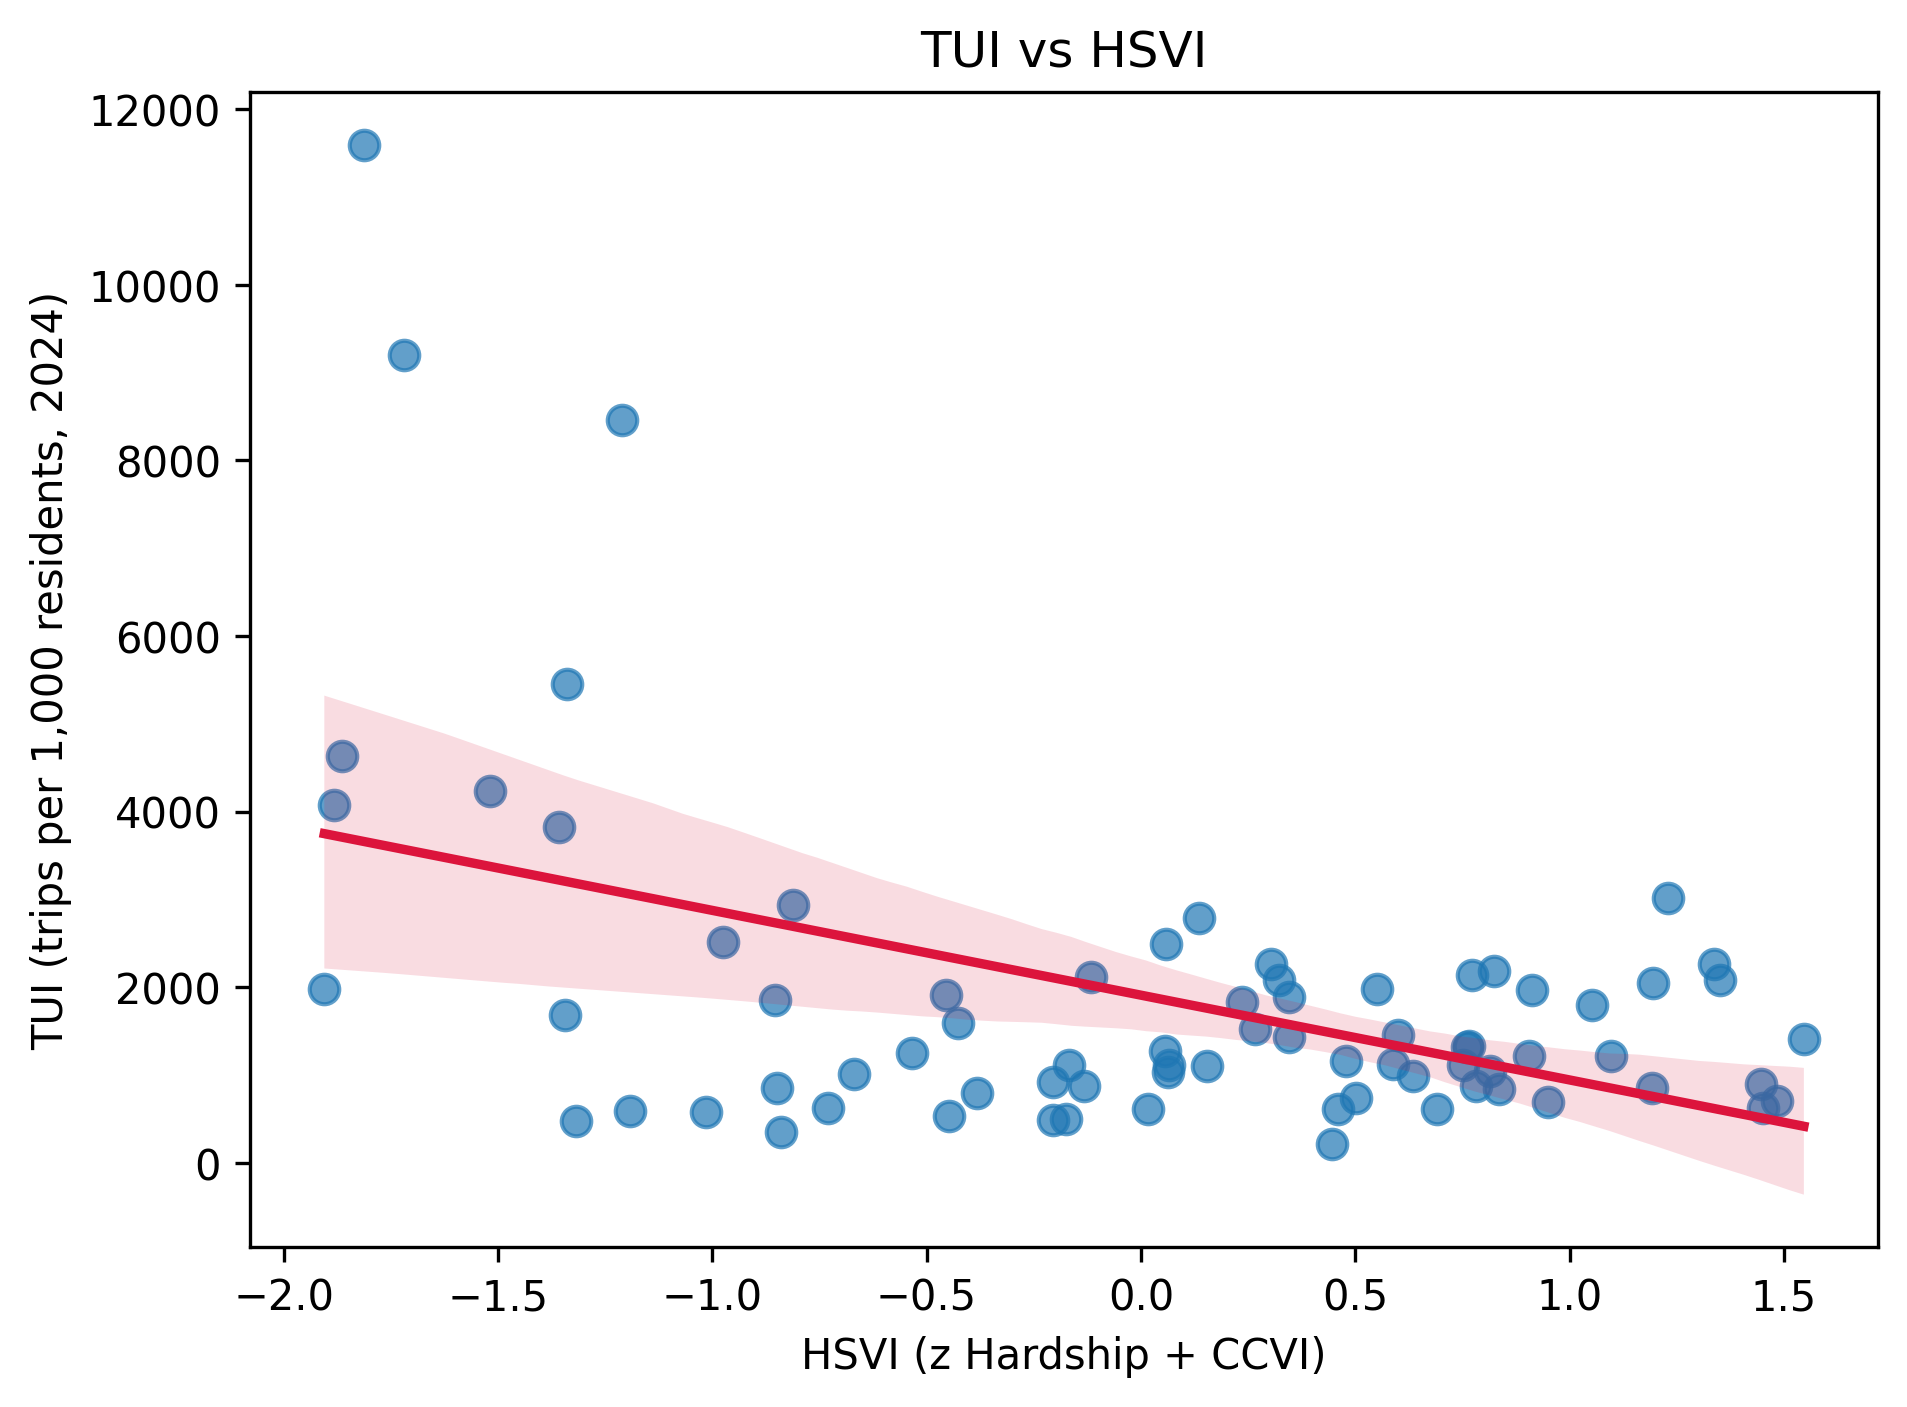
\includegraphics[width=0.55\textwidth]{figs/tui_vs_hsvi_2024.png}
    \caption{TUI vs HSVI, 2024 ($n=75$). Pearson $r=-0.472$, $p<0.001$.}
    \label{fig:scatter_hsvi}
\end{figure}

\begin{figure}[htbp]
    \centering
    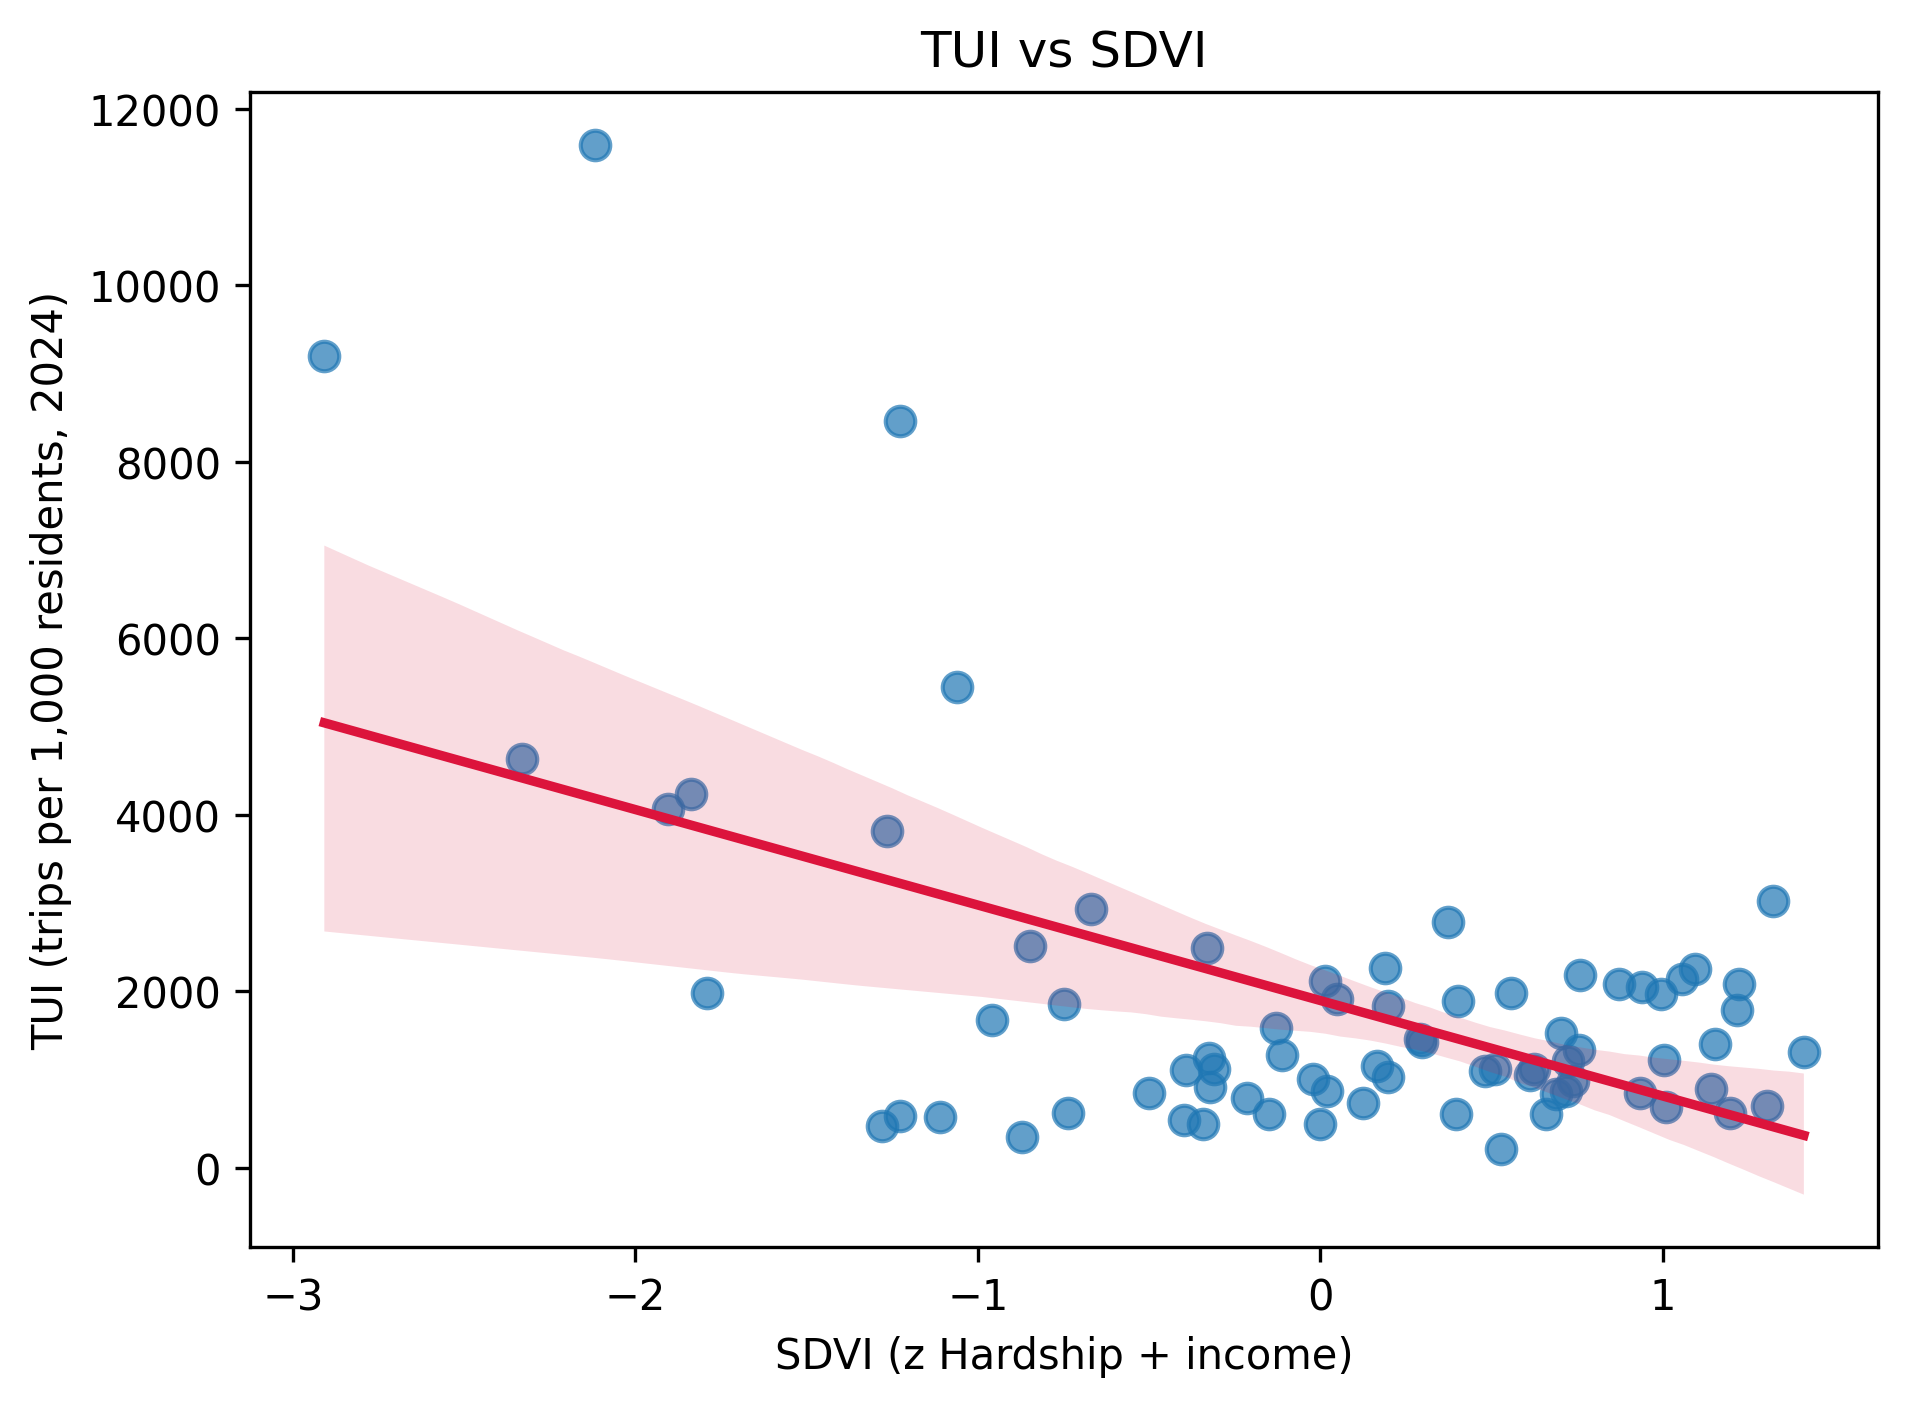
\includegraphics[width=0.55\textwidth]{figs/tui_vs_sdvi_2024.png}
    \caption{TUI vs SDVI, 2024 ($n=75$). Pearson $r=-0.542$, $p<0.001$.}
    \label{fig:scatter_sdvi}
\end{figure}

\begin{table}[htbp]
    \centering
    \caption{TUI (2024) versus vulnerability indicators ($n=75$).}
    \label{tab:corr}
    \begin{tabular}{|l|c|c|c|c|}
        \hline
        \textbf{Indicator} & \textbf{Pearson $r$} & \textbf{$p$} & \textbf{Spearman $\rho$} & \textbf{$p$} \\
        \hline
        HSVI  & $-0.472$ & $<0.001$ & $-0.174$ & $0.134$ \\
        SDVI  & $-0.542$ & $<0.001$ & $-0.120$ & $0.306$ \\
        CCVI  & $-0.515$ & $<0.001$ & $-0.255$ & $0.027$ \\
        \hline
    \end{tabular}
\end{table}

\subsection{Weighted TUI: income-normalised financial burden}
Raw TUI can mislead equity analysis because a moderate trip count in a low-income CA may represent a larger household sacrifice than intense usage in an affluent zone. \textbf{Weighted TUI} normalises estimated annual ridesourcing spend by per capita income:
\begin{equation}
    \mathrm{Weighted\_TUI}_i = \frac{(\text{n\_trips}_{i,2024} \times \text{median\_fare}_i) / \text{population}_i}{\text{per capita income}_i}.
\end{equation}
Annual trips and population come from the monthly TNP merge; \texttt{median\_fare} is queried per pickup CA from 2023--2024 trip records (\texttt{source\_tnp\_fares}). Income is from the hardship release. The indicator answers: \emph{what share of local income is absorbed by origin-area ridesourcing spend?}

Weighted TUI partially inverts the TUI geography (Figure~\ref{fig:wtui}). Fuller Park (CA~37, 0.0039) and Garfield Ridge (CA~56, 0.0037) rank highest despite moderate pickup counts, because median fares and trip volumes consume a larger fraction of local income than in Lincoln Park or the Near North Side. Near West Side (CA~28, 0.0032) and the Loop (CA~32, 0.0032) follow; Riverdale (CA~54, 0.0027) appears in the top tier despite low TUI, reflecting hardship-weighted burden among residents who do use TNP.

Policy implication: subsidies keyed only to pickup heat maps would miss Fuller Park and Garfield Ridge while over-targeting the Loop, where high TUI reflects visitor and commuter demand rather than resident financial stress.

\subsection{Travel time to the Loop}
Chicago's employment and service core remains strongly Loop-oriented. We measure peripherality as the mean \texttt{trip\_seconds} from trip-level TNP records with dropoff in CA~32 (Loop), aggregated by pickup CA for 2024 (\texttt{source\_loop\_travel\_times}). This captures realised ridesourcing travel time to the CBD, not straight-line distance.

Figure~\ref{fig:loop} shows a radial gradient. Mean travel time is about 7.5 minutes from the Loop itself, roughly 10 minutes from Near North and Near West Side, and rises to 43 minutes from Edison Park (CA~9) at the northern edge. Norwood Park, Dunning, and Mount Greenwood exceed 38 minutes. Longer rides compound fare costs for residents who must reach central jobs.

TUI correlates negatively with mean Loop travel time (Pearson $r=-0.67$, $p<0.001$): peripheral origins generate fewer pickups per resident. Travel time also correlates with transit deficit ($r=0.73$), so weak public supply and long radial TNP rides co-occur. Both enter regression as separate z-scored predictors because each captures a distinct facet of peripherality: scheduled CTA supply versus realised private travel time to the core.

\subsection{Transit Accessibility Index (TAI)}
Public transport supply is summarised by a composite \textbf{Transit Accessibility Index} built in \texttt{compute\_transit\_accessibility}. For each CA we compute bus stops per km$^2$ (CTA bus stop layer, spatial join), rail stations per km$^2$ (CTA ``L'' station layer), and weekday GTFS departures per km$^2$ (sum of \texttt{stop\_times} on Wednesday service days from \texttt{data/google\_transit}). Each component is z-scored citywide; TAI is their arithmetic mean. \textbf{Transit deficit} is the negated z-score: $\mathrm{TransitDeficit}_i = -z(\mathrm{TransitAccess}_i)$. Higher deficit means worse combined infrastructure and scheduled frequency.

Including GTFS departures matters because stop density alone can overstate access where buses run infrequently. Riverdale (deficit 1.58), Hegewisch (1.56), South Deering (1.46), and Edison Park (1.43) rank among the most deprived; the Loop shows the strongest supply (Figure~\ref{fig:transit}).

TUI correlates positively with transit access ($r=0.75$) and negatively with deficit ($r=-0.75$). This is the central paradox: ridesourcing intensity co-locates with strong CTA supply, not with its absence. The finding challenges the narrative that TNP primarily substitutes for missing public transport in peripheral hardship zones.

Table~\ref{tab:corr_matrix} reports the full Pearson correlation matrix among TUI and all constructed predictors for 2024. Vulnerability indices correlate positively with transit deficit ($r \approx 0.27$--$0.36$) and with Loop travel time ($r \approx 0.11$--$0.26$), but TUI moves in the opposite direction to vulnerability and travel time while tracking transit access.

\begin{table}[htbp]
    \centering
    \caption{Pearson correlation matrix, 2024 ($n=75$).}
    \label{tab:corr_matrix}
    \small
    \begin{tabular}{|l|r|r|r|r|r|}
        \hline
        & \textbf{TUI} & \textbf{HSVI} & \textbf{SDVI} & \textbf{Transit acc.} & \textbf{Loop time} \\
        \hline
        TUI            &  1.000 & $-0.472$ & $-0.542$ &  0.749 & $-0.672$ \\
        HSVI           & $-0.472$ &  1.000 &  0.960 & $-0.269$ &  0.110 \\
        SDVI           & $-0.542$ &  0.960 &  1.000 & $-0.283$ &  0.111 \\
        Transit access &  0.749 & $-0.269$ & $-0.283$ &  1.000 & $-0.730$ \\
        Transit deficit& $-0.749$ &  0.269 &  0.283 & $-1.000$ &  0.730 \\
        Loop time (s)  & $-0.672$ &  0.110 &  0.111 & $-0.730$ &  1.000 \\
        \hline
    \end{tabular}
\end{table}

\subsection{Temporal comparison: 2018 versus 2024}\label{sec:temporal}
Monthly TNP counts span 2018--2019 and 2023--2024 in our cached extracts (the legacy 2018--2022 portal release contributes 2018--2019; 2020--2022 are absent from the local cache, likely reflecting reporting gaps during the COVID-19 period). We therefore compare the earliest available year (2018) with the reference year (2024) to assess whether the core--periphery gradient persisted or shifted.

Figures~\ref{fig:tui2018} and~\ref{fig:tui} show median annual TUI choropleths. Table~\ref{tab:temporal_top} lists the five highest-TUI CAs in each year; Table~\ref{tab:temporal_change} reports the largest relative changes. Citywide median TUI was 1{,}105 per 1{,}000 residents in 2018 and 1{,}296 in 2024 (mean 2{,}498 $\to$ 2{,}124). Spearman rank correlation across CAs is $\rho=0.89$ ($p<0.001$): the \emph{relative} ordering of neighbourhoods is highly stable.

Two patterns coexist. First, \textbf{geographic ranking persists}: the Loop, Near North Side, and Near West Side lead in both years; East Side and Hegewisch remain among the lowest. The 2024 cross-sectional equity findings are not an artefact of a single post-pandemic year. Second, \textbf{levels changed unevenly}: central CAs saw large \emph{declines} in absolute TUI (Loop $-47.5\%$, Near North Side $-46.0\%$, West Town $-41.9\%$), while several South Side peripheries \emph{grew} from a low base (Riverdale $+123\%$, West Pullman $+101\%$, Hegewisch $+94\%$). Hyde Park enters the 2024 top five (5{,}451) replacing Near South Side.

This temporal evidence does not overturn the rejected compensatory hypothesis. Even after faster peripheral growth, 2024 TUI in Riverdale (1{,}317) remains an order of magnitude below the Loop (11{,}596). Regression and vulnerability correlations are estimated for 2024 because fare, Loop travel-time, and GTFS fields exist only for recent years; the 2018--2024 comparison is descriptive stability and level change, not a panel model.

\begin{figure}[htbp]
    \centering
    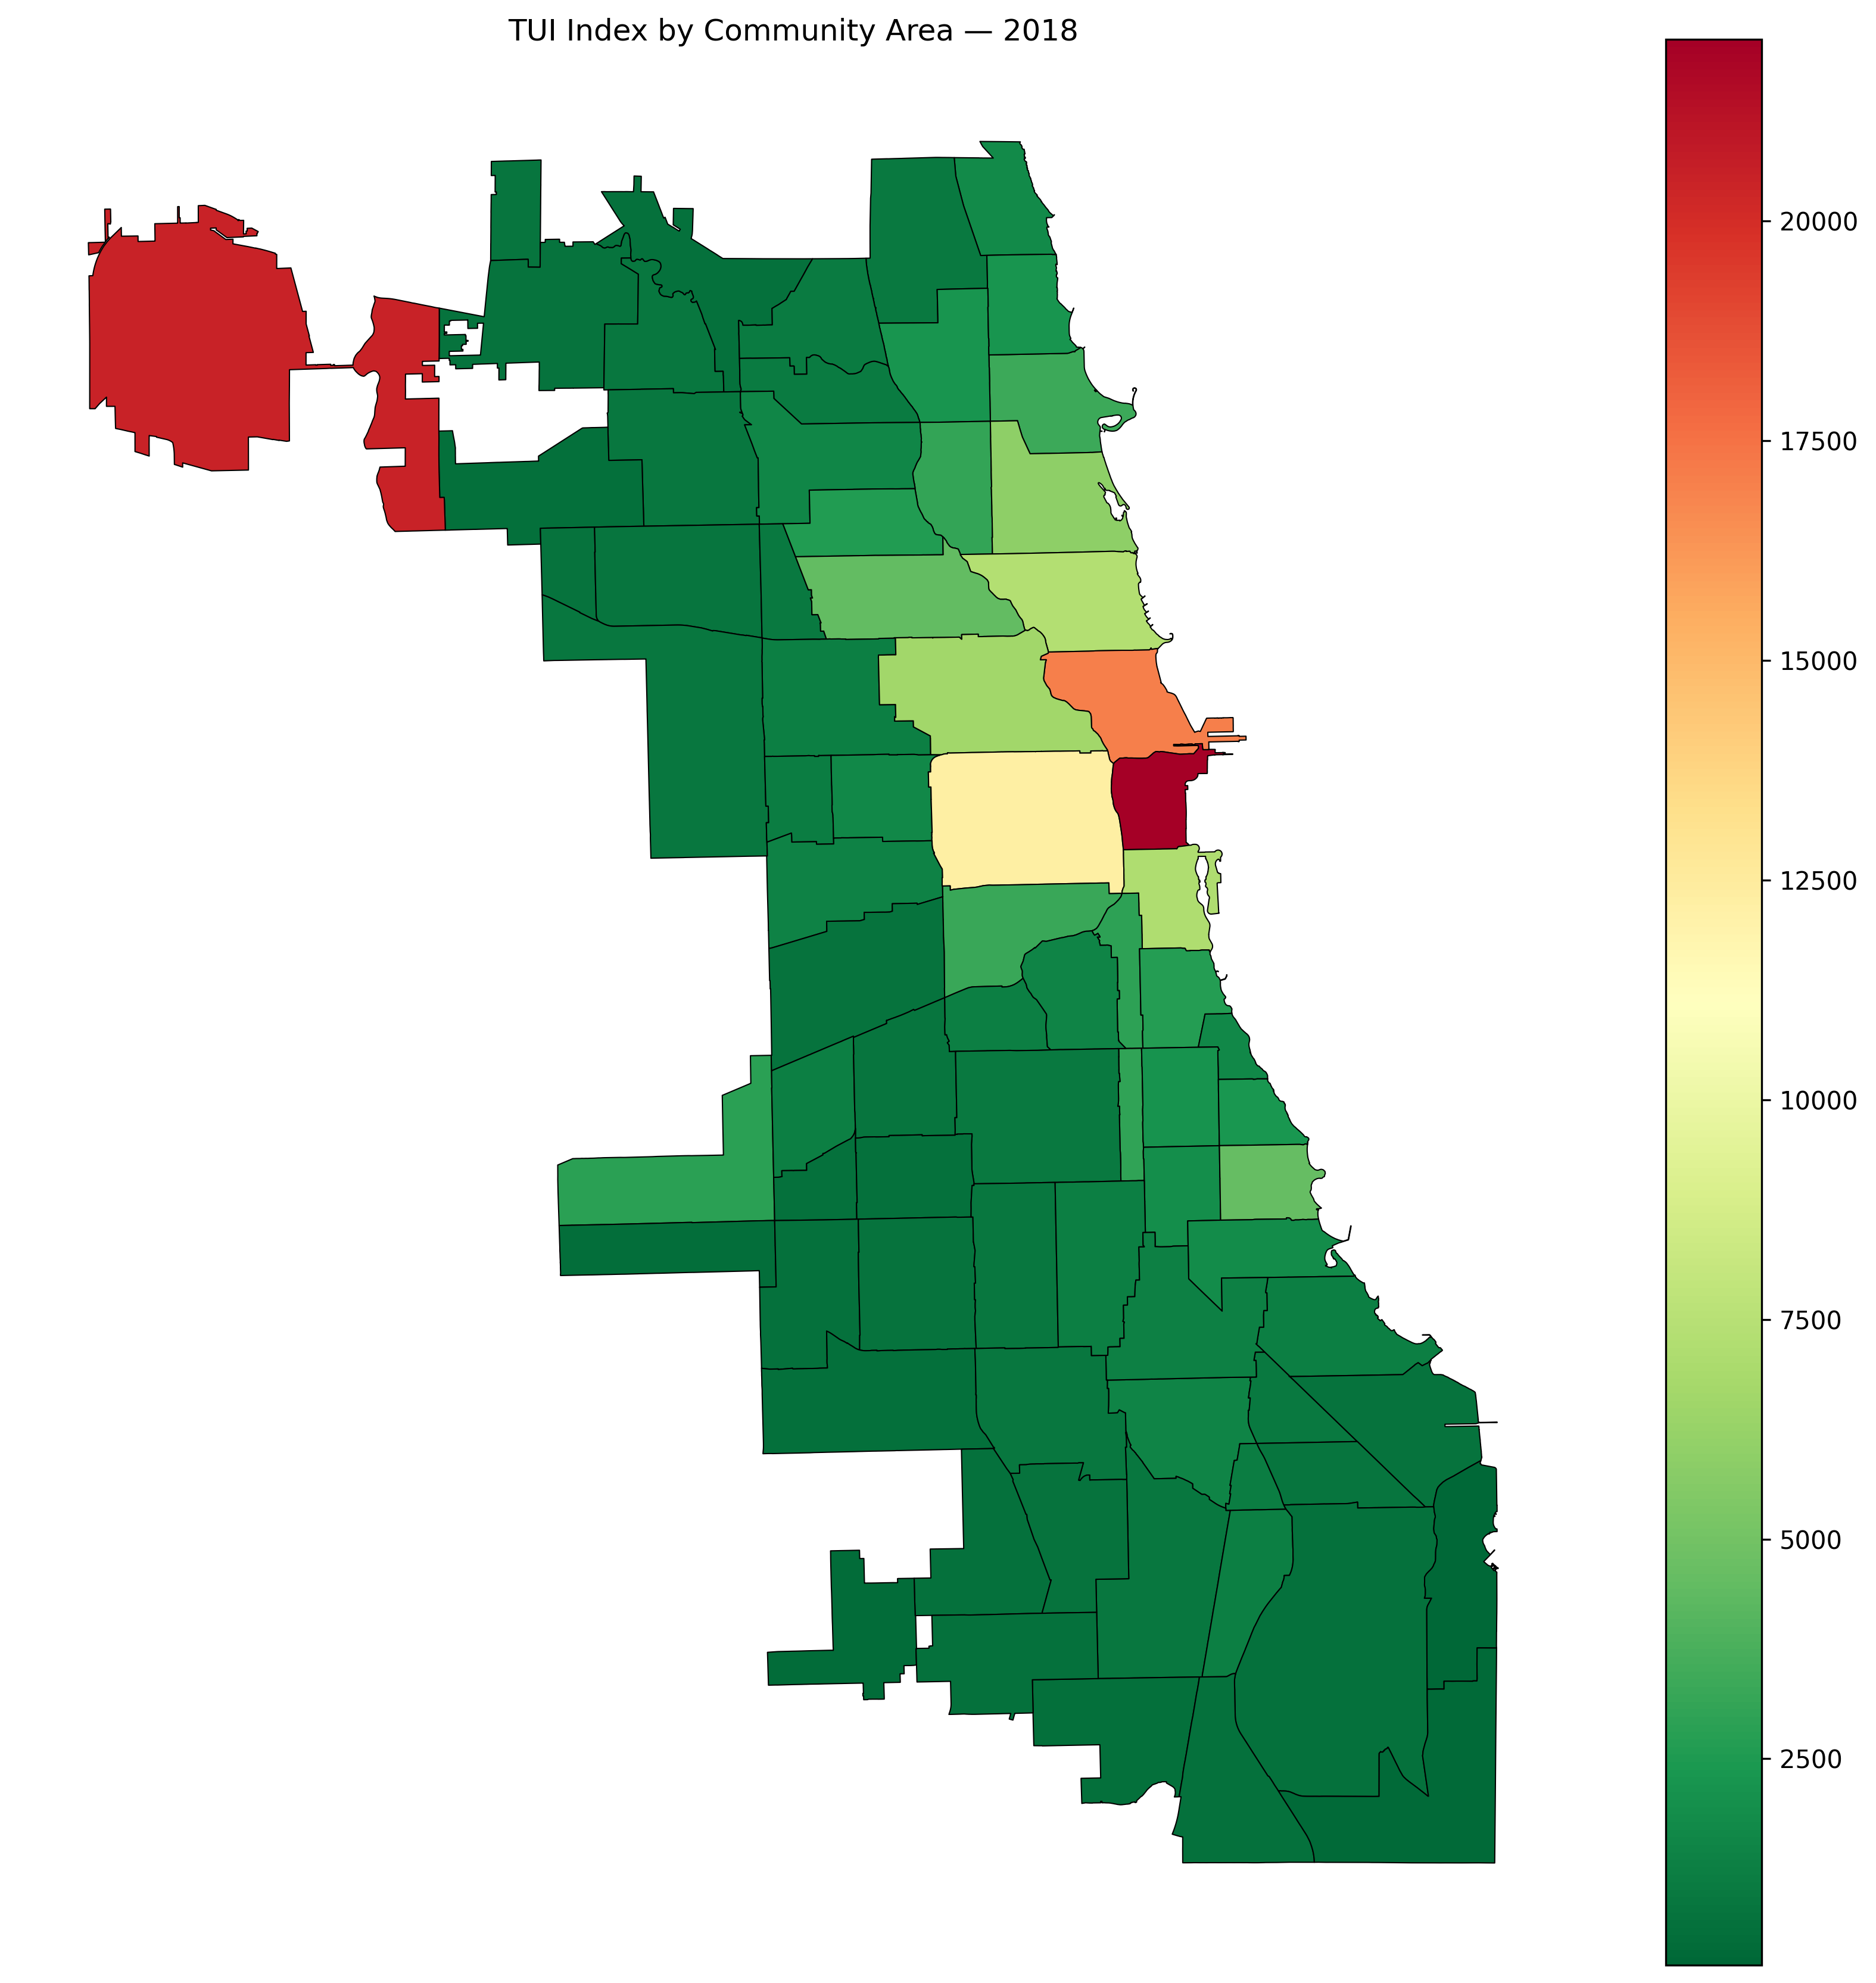
\includegraphics[width=0.48\textwidth]{figs/tui_2018.png}
    \caption{Median annual TUI by Community Area, 2018.}
    \label{fig:tui2018}
\end{figure}

\begin{table}[htbp]
    \centering
    \caption{Top five CAs by median TUI, 2018 vs.\ 2024.}
    \label{tab:temporal_top}
    \small
    \begin{tabular}{|l|r||l|r|}
        \hline
        \textbf{2018} & \textbf{TUI} & \textbf{2024} & \textbf{TUI} \\
        \hline
        Loop & 22{,}069 & Loop & 11{,}596 \\
        Near North Side & 17{,}026 & Near North Side & 9{,}196 \\
        Near West Side & 12{,}271 & Near West Side & 8{,}461 \\
        Lincoln Park & 7{,}272 & Hyde Park & 5{,}451 \\
        Near South Side & 7{,}157 & Lincoln Park & 4{,}628 \\
        \hline
    \end{tabular}
\end{table}

\begin{table}[htbp]
    \centering
    \caption{Largest relative TUI changes, 2018$\to$2024 (median annual).}
    \label{tab:temporal_change}
    \small
    \begin{tabular}{|l|r|r|r|}
        \hline
        \textbf{Community Area} & \textbf{2018} & \textbf{2024} & \textbf{Change (\%)} \\
        \hline
        \multicolumn{4}{|l|}{\textit{Largest increases}} \\
        \hline
        Riverdale & 590 & 1{,}317 & $+123$ \\
        West Pullman & 559 & 1{,}122 & $+101$ \\
        Hegewisch & 254 & 494 & $+94$ \\
        Pullman & 1{,}209 & 2{,}260 & $+87$ \\
        Burnside & 1{,}105 & 2{,}047 & $+85$ \\
        \hline
        \multicolumn{4}{|l|}{\textit{Largest decreases}} \\
        \hline
        Loop & 22{,}069 & 11{,}596 & $-48$ \\
        Near North Side & 17{,}026 & 9{,}196 & $-46$ \\
        West Town & 6{,}574 & 3{,}823 & $-42$ \\
        Near South Side & 7{,}157 & 4{,}237 & $-41$ \\
        Lincoln Park & 7{,}272 & 4{,}628 & $-36$ \\
        \hline
    \end{tabular}
\end{table}

\subsection{Spatial autocorrelation: Moran's I and LISA}
\subsubsection{Global clustering: Moran's $I$}
TUI exhibits strong positive spatial autocorrelation. Moran's $I=0.61$ ($p=0.001$, 999 permutations) on Queen-contiguity weights ($n=75$): neighbouring CAs tend to share similar intensity more than a random spatial permutation would predict. The Moran scatterplot relates each CA's standardised TUI to the average standardised TUI of Queen neighbours (shared border or vertex). The positive slope confirms that high-TUI areas cluster together spatially, consistent with land-use and activity patterns rather than isolated outliers.

\subsubsection{Local clusters: LISA}
Local Indicators of Spatial Association (LISA) classify each CA into five categories at $p<0.05$: High--High (hot spots), Low--Low (cold spots), High--Low and Low--High (spatial outliers), or not significant. Figure~\ref{fig:lisa} maps the result; Table~\ref{tab:lisa} lists significant CAs.

The High--High cluster ($n=7$) forms a contiguous core: Loop (TUI 11{,}596), Near North Side (9{,}196), Near West Side (8{,}461), Lincoln Park, Near South Side, West Town, and Armour Square. These zones share intense ridesourcing surrounded by equally intense neighbours.

The Low--Low cluster ($n=13$) spans southwest and northwest residential areas: Morgan Park, Jefferson Park, Chicago Lawn, Belmont Cragin, Portage Park, Brighton Park, Gage Park, Norwood Park, West Elsdon, Ashburn, West Lawn, Beverly, and Forest Glen. Intensity is systematically low and neighbours are similarly low.

Only one spatial outlier is significant: \textbf{Garfield Ridge} (High--Low), with elevated TUI (2{,}491) surrounded by lower-intensity neighbours. This aligns with Weighted TUI ranking Garfield Ridge among the highest burden zones: a pocket of relatively higher usage and spend in a moderate-intensity border context.

Notably, far South Side areas with very low TUI (Riverdale, East Side, Hegewisch) do \emph{not} reach LISA significance at $p=0.05$: their low intensity is extreme but spatial inference is limited by neighbour configuration and sample size at the ecological scale. Moran's $I$ nonetheless confirms citywide clustering; LISA localises where that clustering is statistically robust.

\begin{figure}[htbp]
    \centering
    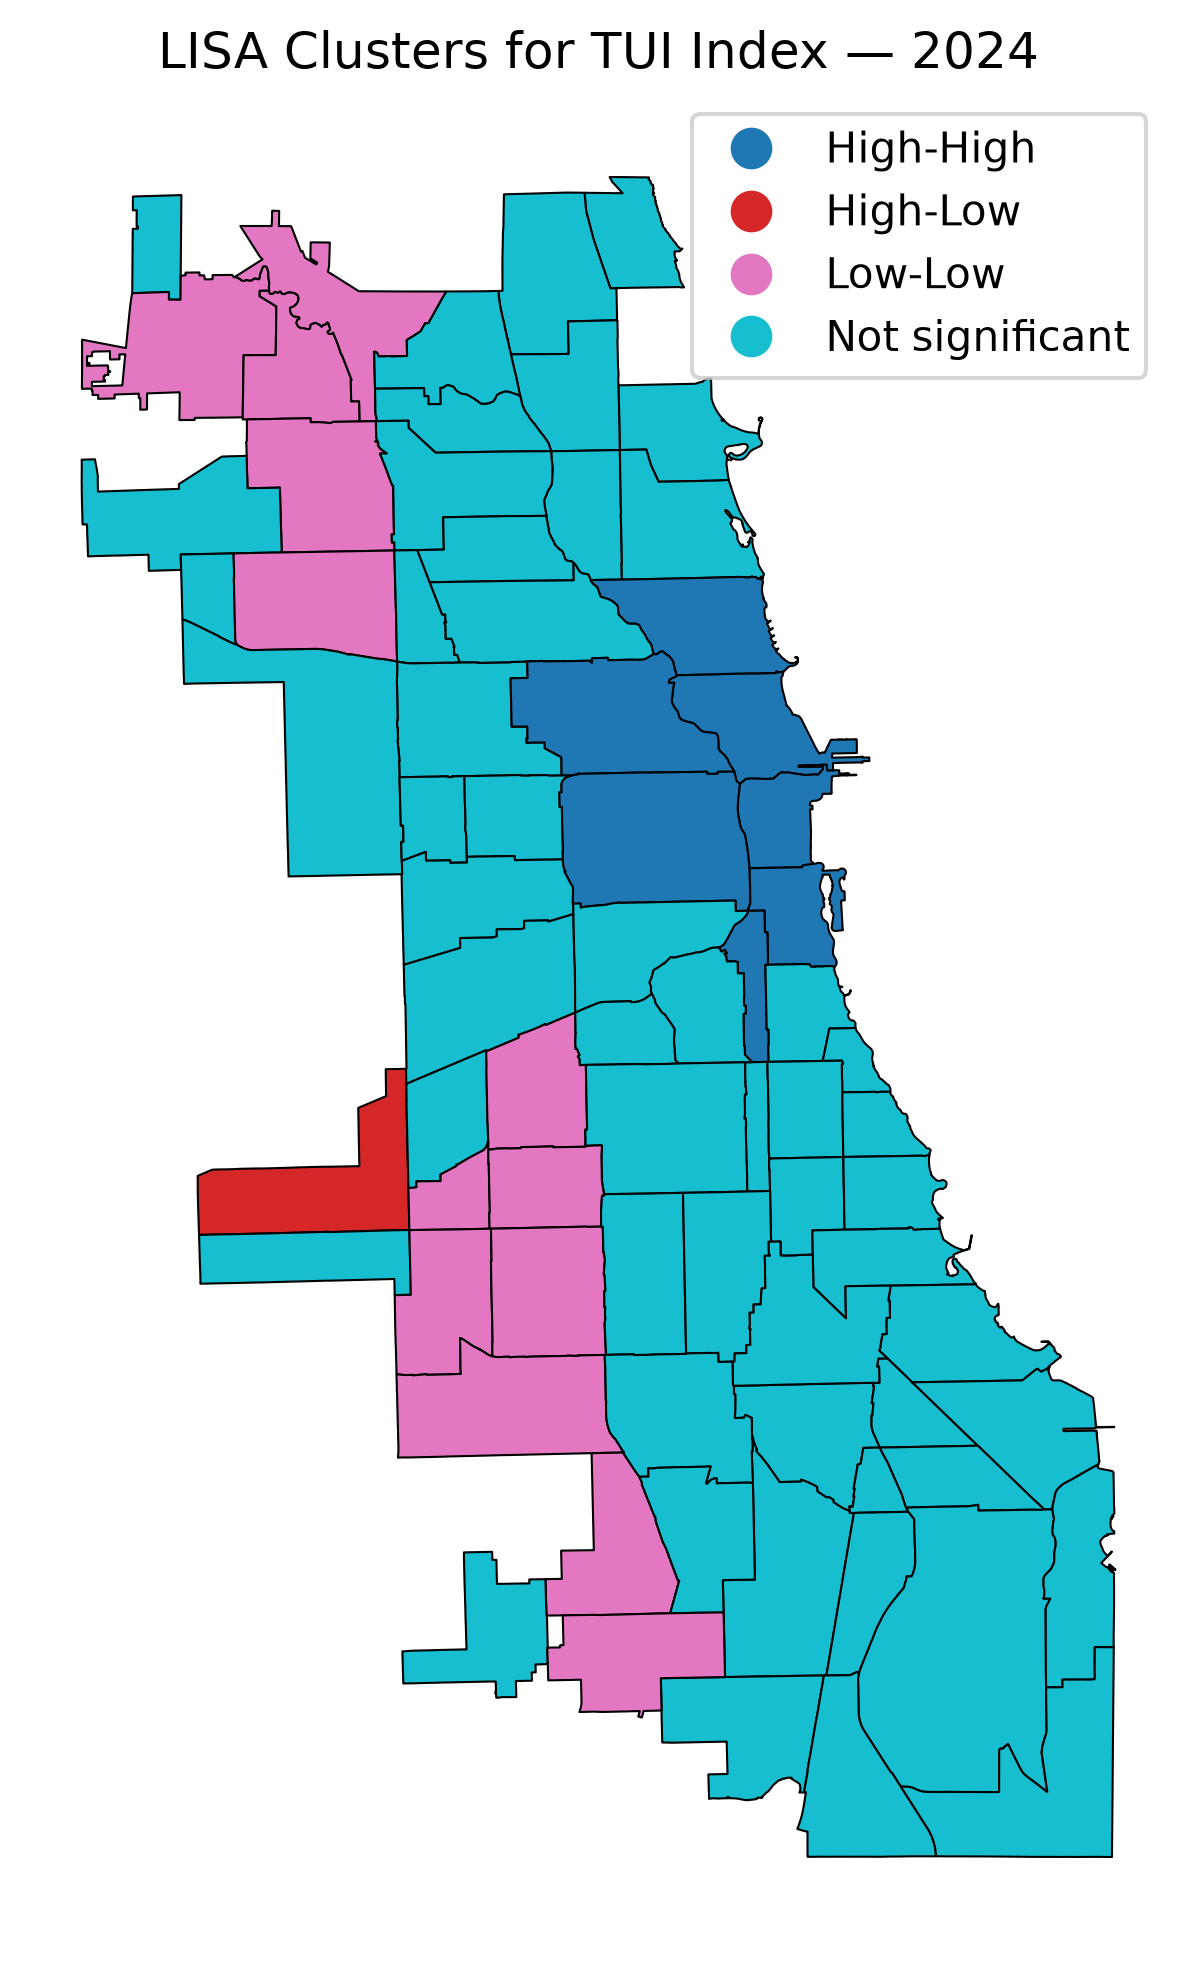
\includegraphics[width=0.62\textwidth]{figs/lisa_tui_2024.png}
    \caption{LISA clusters for median TUI, 2024 ($n=75$, Queen weights, $p<0.05$).}
    \label{fig:lisa}
\end{figure}

\begin{table}[htbp]
    \centering
    \caption{Significant LISA clusters for TUI, 2024.}
    \label{tab:lisa}
    \small
    \begin{tabular}{|l|l|r|}
        \hline
        \textbf{Cluster} & \textbf{Community Area} & \textbf{TUI} \\
        \hline
        \multirow{7}{*}{High--High} & Loop (32) & 11{,}596 \\
        & Near North Side (8) & 9{,}196 \\
        & Near West Side (28) & 8{,}461 \\
        & Lincoln Park (7) & 4{,}628 \\
        & Near South Side (33) & 4{,}237 \\
        & West Town (24) & 3{,}823 \\
        & Armour Square (34) & 2{,}078 \\
        \hline
        \multirow{5}{*}{Low--Low (sample)} & Morgan Park (75) & 1{,}110 \\
        & Chicago Lawn (66) & 846 \\
        & Brighton Park (58) & 690 \\
        & Norwood Park (10) & 625 \\
        & Forest Glen (12) & 474 \\
        \hline
        High--Low & Garfield Ridge (56) & 2{,}491 \\
        \hline
    \end{tabular}
\end{table}

\subsection{Regression analysis}
\subsubsection{Model specification}
The dependent variable is $y_i = \log(1+\mathrm{TUI}_i)$ (Equation~2). Predictors are z-scored (Equation~1): transit deficit, HSVI, and mean Loop travel time (seconds). We use HSVI rather than SDVI because HSVI is the project baseline (hardship + CCVI) and SDVI overlaps with income-based Weighted TUI ($r=0.96$ between HSVI and SDVI). Spatial models follow Equations~(7)--(8); selection uses AIC (Equation~9).

\subsubsection{Ordinary Least Squares}
OLS with HC3 heteroskedasticity-robust standard errors explains 68.9\% of variance in $\log(1+\mathrm{TUI})$ (Table~\ref{tab:ols}). All three predictors enter negatively: higher transit deficit ($\beta=-0.178$, $p=0.020$), HSVI ($\beta=-0.153$, $p=0.002$), and Loop travel time ($\beta=-0.436$, $p<0.001$) associate with lower logged TUI. A one-SD increase in travel time corresponds to roughly a 36\% decrease in $(1+\mathrm{TUI})$ holding other predictors fixed ($e^{-0.436}-1 \approx -0.35$).

Despite good fit, residual Moran's $I=0.27$ ($p=0.001$) indicates remaining spatial structure in OLS errors: neighbouring CAs share unmodelled similarity beyond what predictors capture. This motivates explicit spatial models \cite{anselin1988}.

\subsubsection{Spatial Error Model versus Spatial Lag Model}
We compare SEM (Equation~7) and SLAG (Equation~8) on the same $n=75$ sample with row-standardised Queen weights. SEM is appropriate when spatial shocks propagate through errors; SLAG when neighbours' TUI directly affects local intensity.

SEM is preferred by Akaike Information Criterion: AIC 75.2 versus 80.0 for SLAG (full model SEM AIC $\approx 74.4$). After SEM filtering, residual Moran's $I$ falls to 0.025 ($p=0.32$), indicating that spatial structure is adequately modelled. SLAG residual Moran's $I$ remains 0.066 ($p<0.05$).

Table~\ref{tab:sem} reports the preferred SEM. HSVI ($\beta=-0.131$, $p=0.030$) and travel time ($\beta=-0.525$, $p<0.001$) remain significant; transit deficit loses significance ($\beta=-0.098$, $p=0.147$), partly because it shares variance with travel time ($r=0.73$) and spatial filtering reallocates explanatory power ($\lambda=0.560$, $p<0.001$). The negative HSVI coefficient confirms that, conditional on peripherality and transit supply, more vulnerable CAs have lower logged TUI. Travel time carries the largest coefficient, emphasising radial distance to the Loop as the strongest suppressor of intensity.

Table~\ref{tab:slag} summarises SLAG for comparison. The spatial autoregressive parameter $\rho=0.44$ is significant, but worse AIC and residual autocorrelation favour SEM for inference.

\subsubsection{Robustness and diagnostics}
Appendix~A of the notebook reports variance inflation factors (all below conventional thresholds of 5) and reduced models dropping travel time. Reduced specifications sharply worsen AIC (SEM $\approx 96$, SLAG $\approx 88$), confirming that travel time is not redundant despite correlation with deficit. In reduced spatial models the SEM versus SLAG ranking can flip; the full model is therefore retained for the main conclusions.

\begin{table}[htbp]
    \centering
    \caption{OLS on $\log(1+\mathrm{TUI})$ with z-standardised predictors (HC3, $n=75$).}
    \label{tab:ols}
    \begin{tabular}{|l|c|c|}
        \hline
        \textbf{Predictor} & \textbf{Coefficient} & \textbf{$p$-value} \\
        \hline
        Transit deficit (z)   & $-0.178$ & $0.020$ \\
        HSVI (z)              & $-0.153$ & $0.002$ \\
        Mean travel time (z)  & $-0.436$ & $<0.001$ \\
        \hline
        \multicolumn{3}{|l|}{$R^2 = 0.689$; residual Moran's $I = 0.27$ ($p = 0.001$)} \\
        \hline
    \end{tabular}
\end{table}

\begin{table}[htbp]
    \centering
    \caption{Spatial Error Model on $\log(1+\mathrm{TUI})$ ($n=75$).}
    \label{tab:sem}
    \begin{tabular}{|l|c|c|}
        \hline
        \textbf{Predictor} & \textbf{Coefficient} & \textbf{$p$-value} \\
        \hline
        Transit deficit (z)   & $-0.098$ & $0.147$ \\
        HSVI (z)              & $-0.131$ & $0.030$ \\
        Mean travel time (z)  & $-0.525$ & $<0.001$ \\
        Spatial $\lambda$     & $0.560$  & $<0.001$ \\
        \hline
        \multicolumn{3}{|l|}{AIC $= 75.2$; filtered residual Moran's $I = 0.025$ ($p = 0.321$)} \\
        \hline
    \end{tabular}
\end{table}

\begin{table}[htbp]
    \centering
    \caption{Spatial Lag Model on $\log(1+\mathrm{TUI})$ ($n=75$).}
    \label{tab:slag}
    \begin{tabular}{|l|c|c|}
        \hline
        \textbf{Predictor} & \textbf{Coefficient} & \textbf{$p$-value} \\
        \hline
        Transit deficit (z)   & $-0.113$ & $0.092$ \\
        HSVI (z)              & $-0.103$ & $0.030$ \\
        Mean travel time (z)  & $-0.270$ & $0.001$ \\
        Spatial $\rho$        & $0.440$  & $<0.001$ \\
        \hline
        \multicolumn{3}{|l|}{AIC $= 80.0$; residual Moran's $I = 0.066$ ($p < 0.05$)} \\
        \hline
    \end{tabular}
\end{table}

\paragraph{Data visualisation.}
Figures~\ref{fig:tui}--\ref{fig:transit} provide choropleth views of the indicators discussed above. Figure~\ref{fig:tui} maps median 2024 TUI; Figure~\ref{fig:maps} places TUI beside SDVI; Figures~\ref{fig:wtui},~\ref{fig:loop}, and~\ref{fig:transit} map Weighted TUI, Loop travel time, and transit deficit respectively. Together with the LISA map (Figure~\ref{fig:lisa}) and scatterplots (Figures~\ref{fig:scatter_hsvi}--\ref{fig:scatter_sdvi}), they form the geographic narrative supporting the statistical results.

\begin{figure}[htbp]
    \centering
    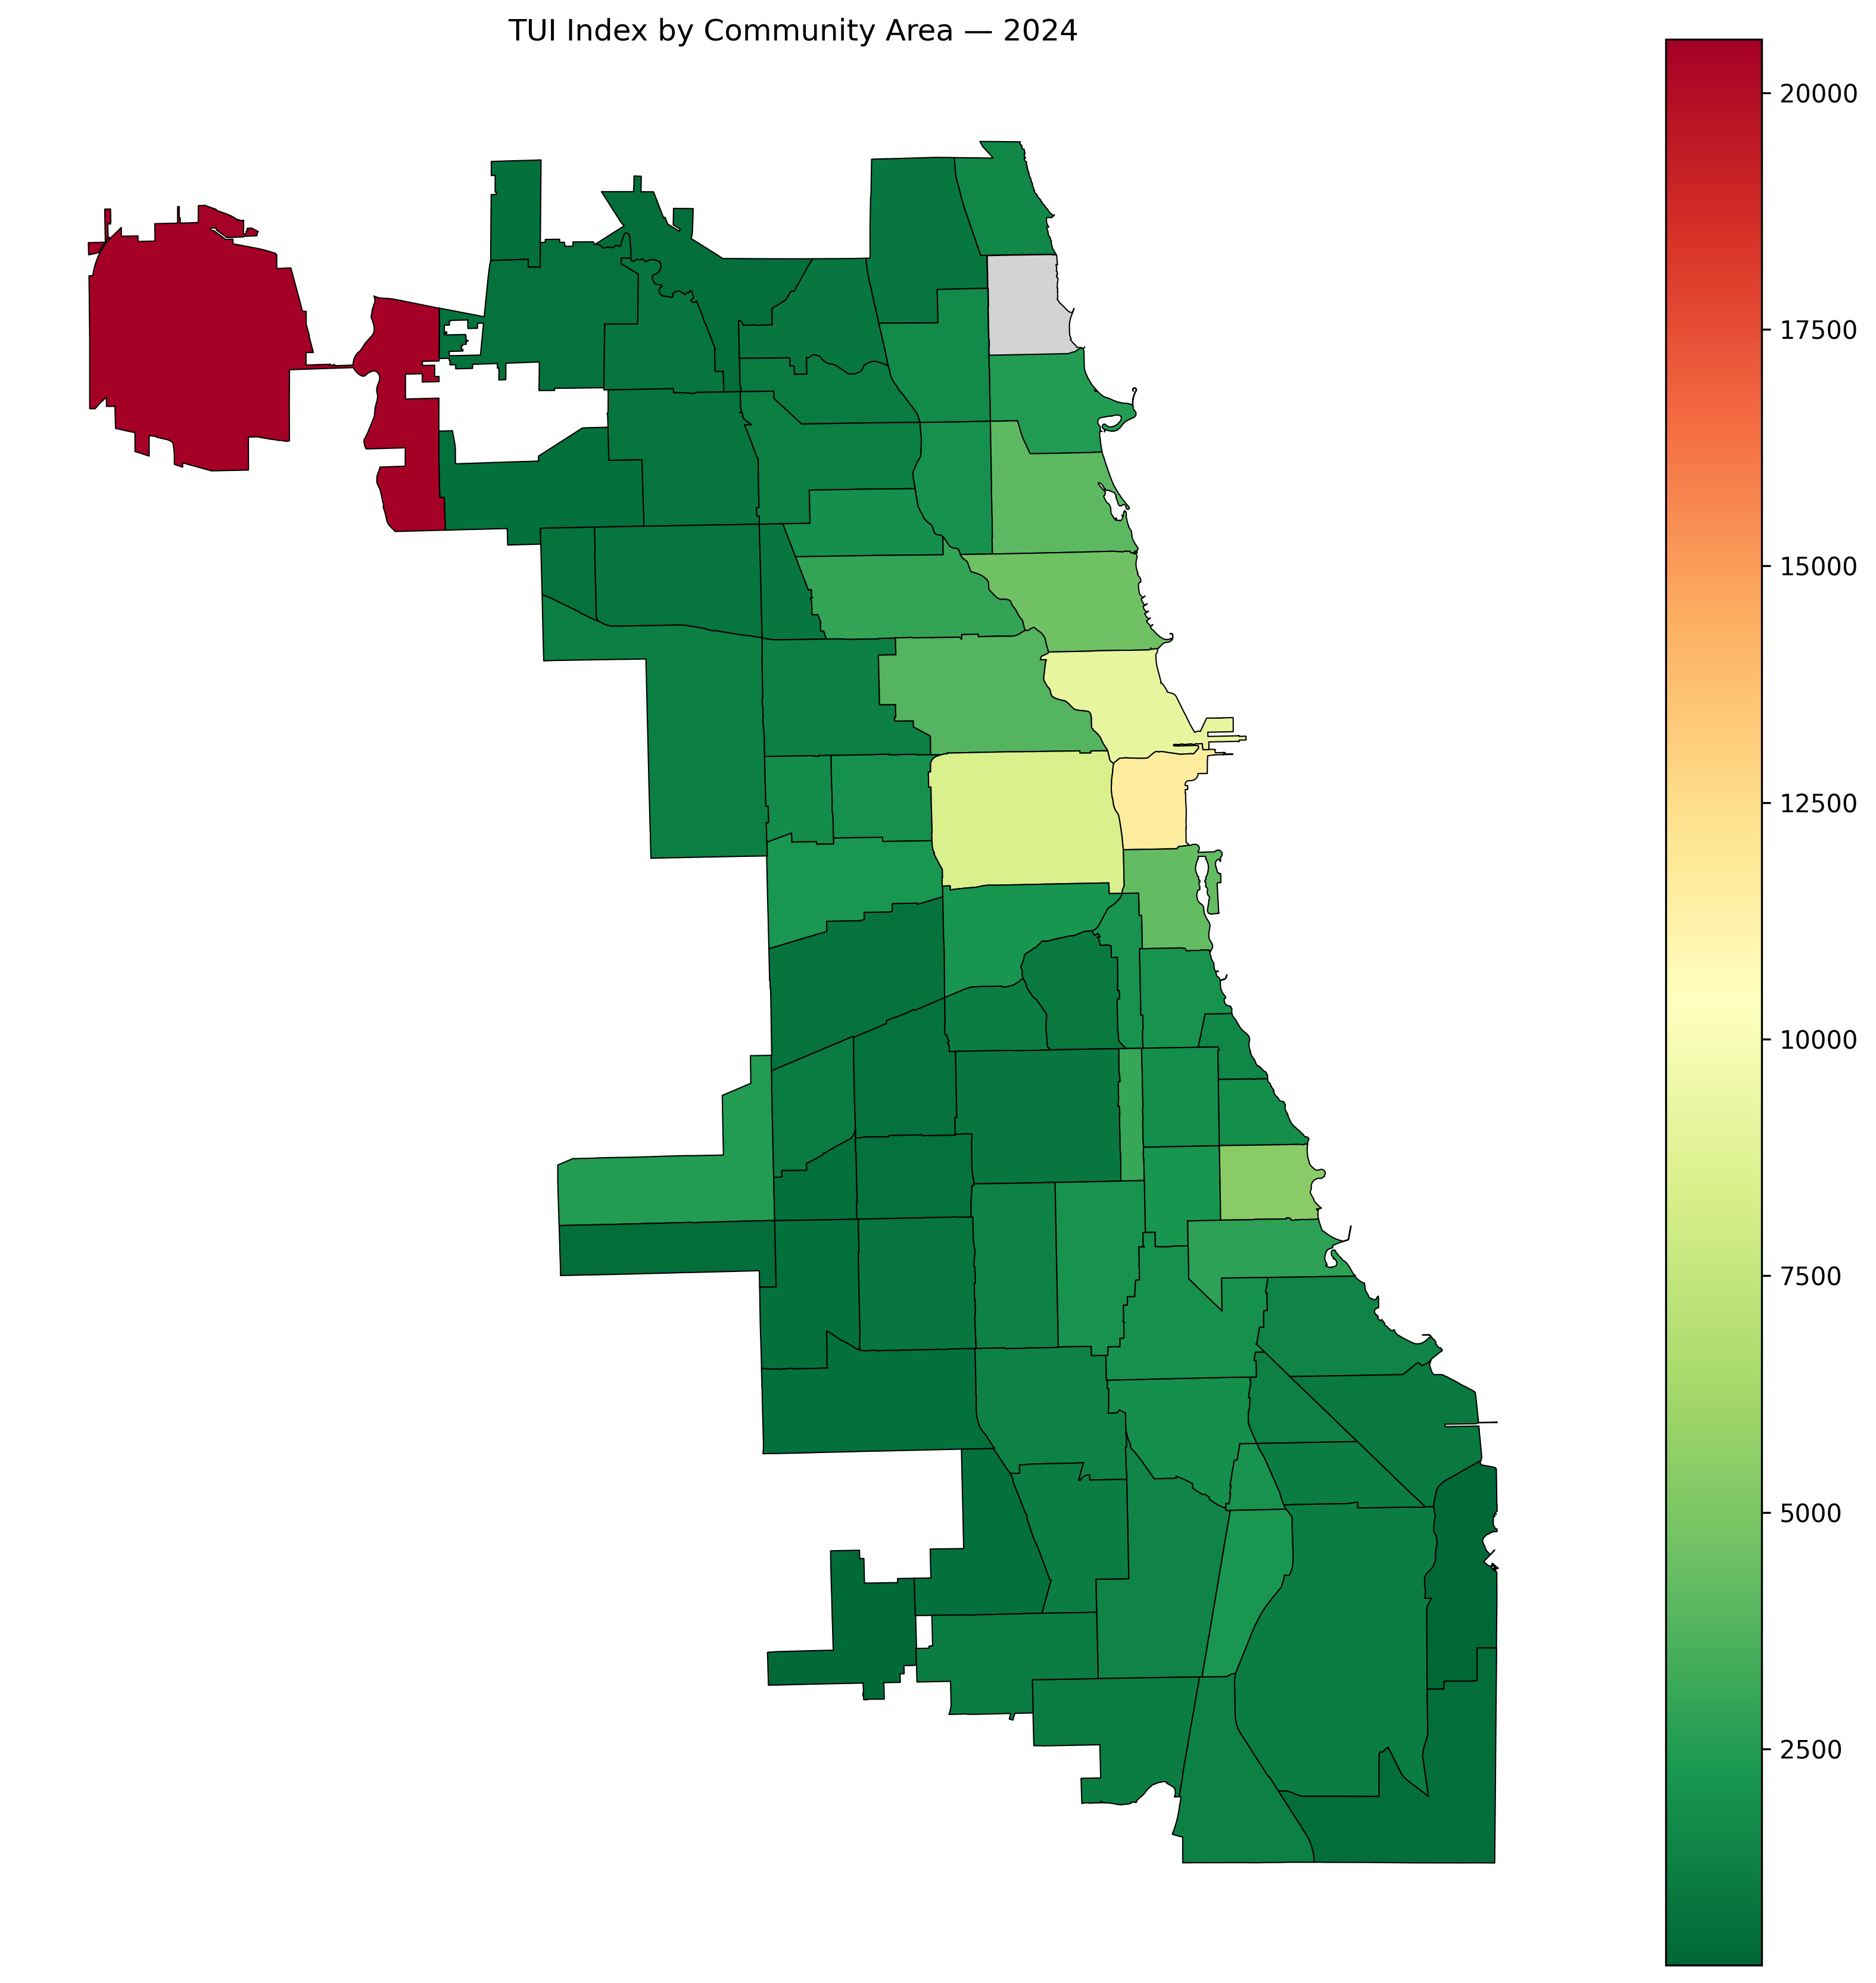
\includegraphics[width=0.48\textwidth]{figs/tui_2024.png}
    \caption{Median annual TUI by Community Area, 2024.}
    \label{fig:tui}
\end{figure}

\begin{figure}[htbp]
    \centering
    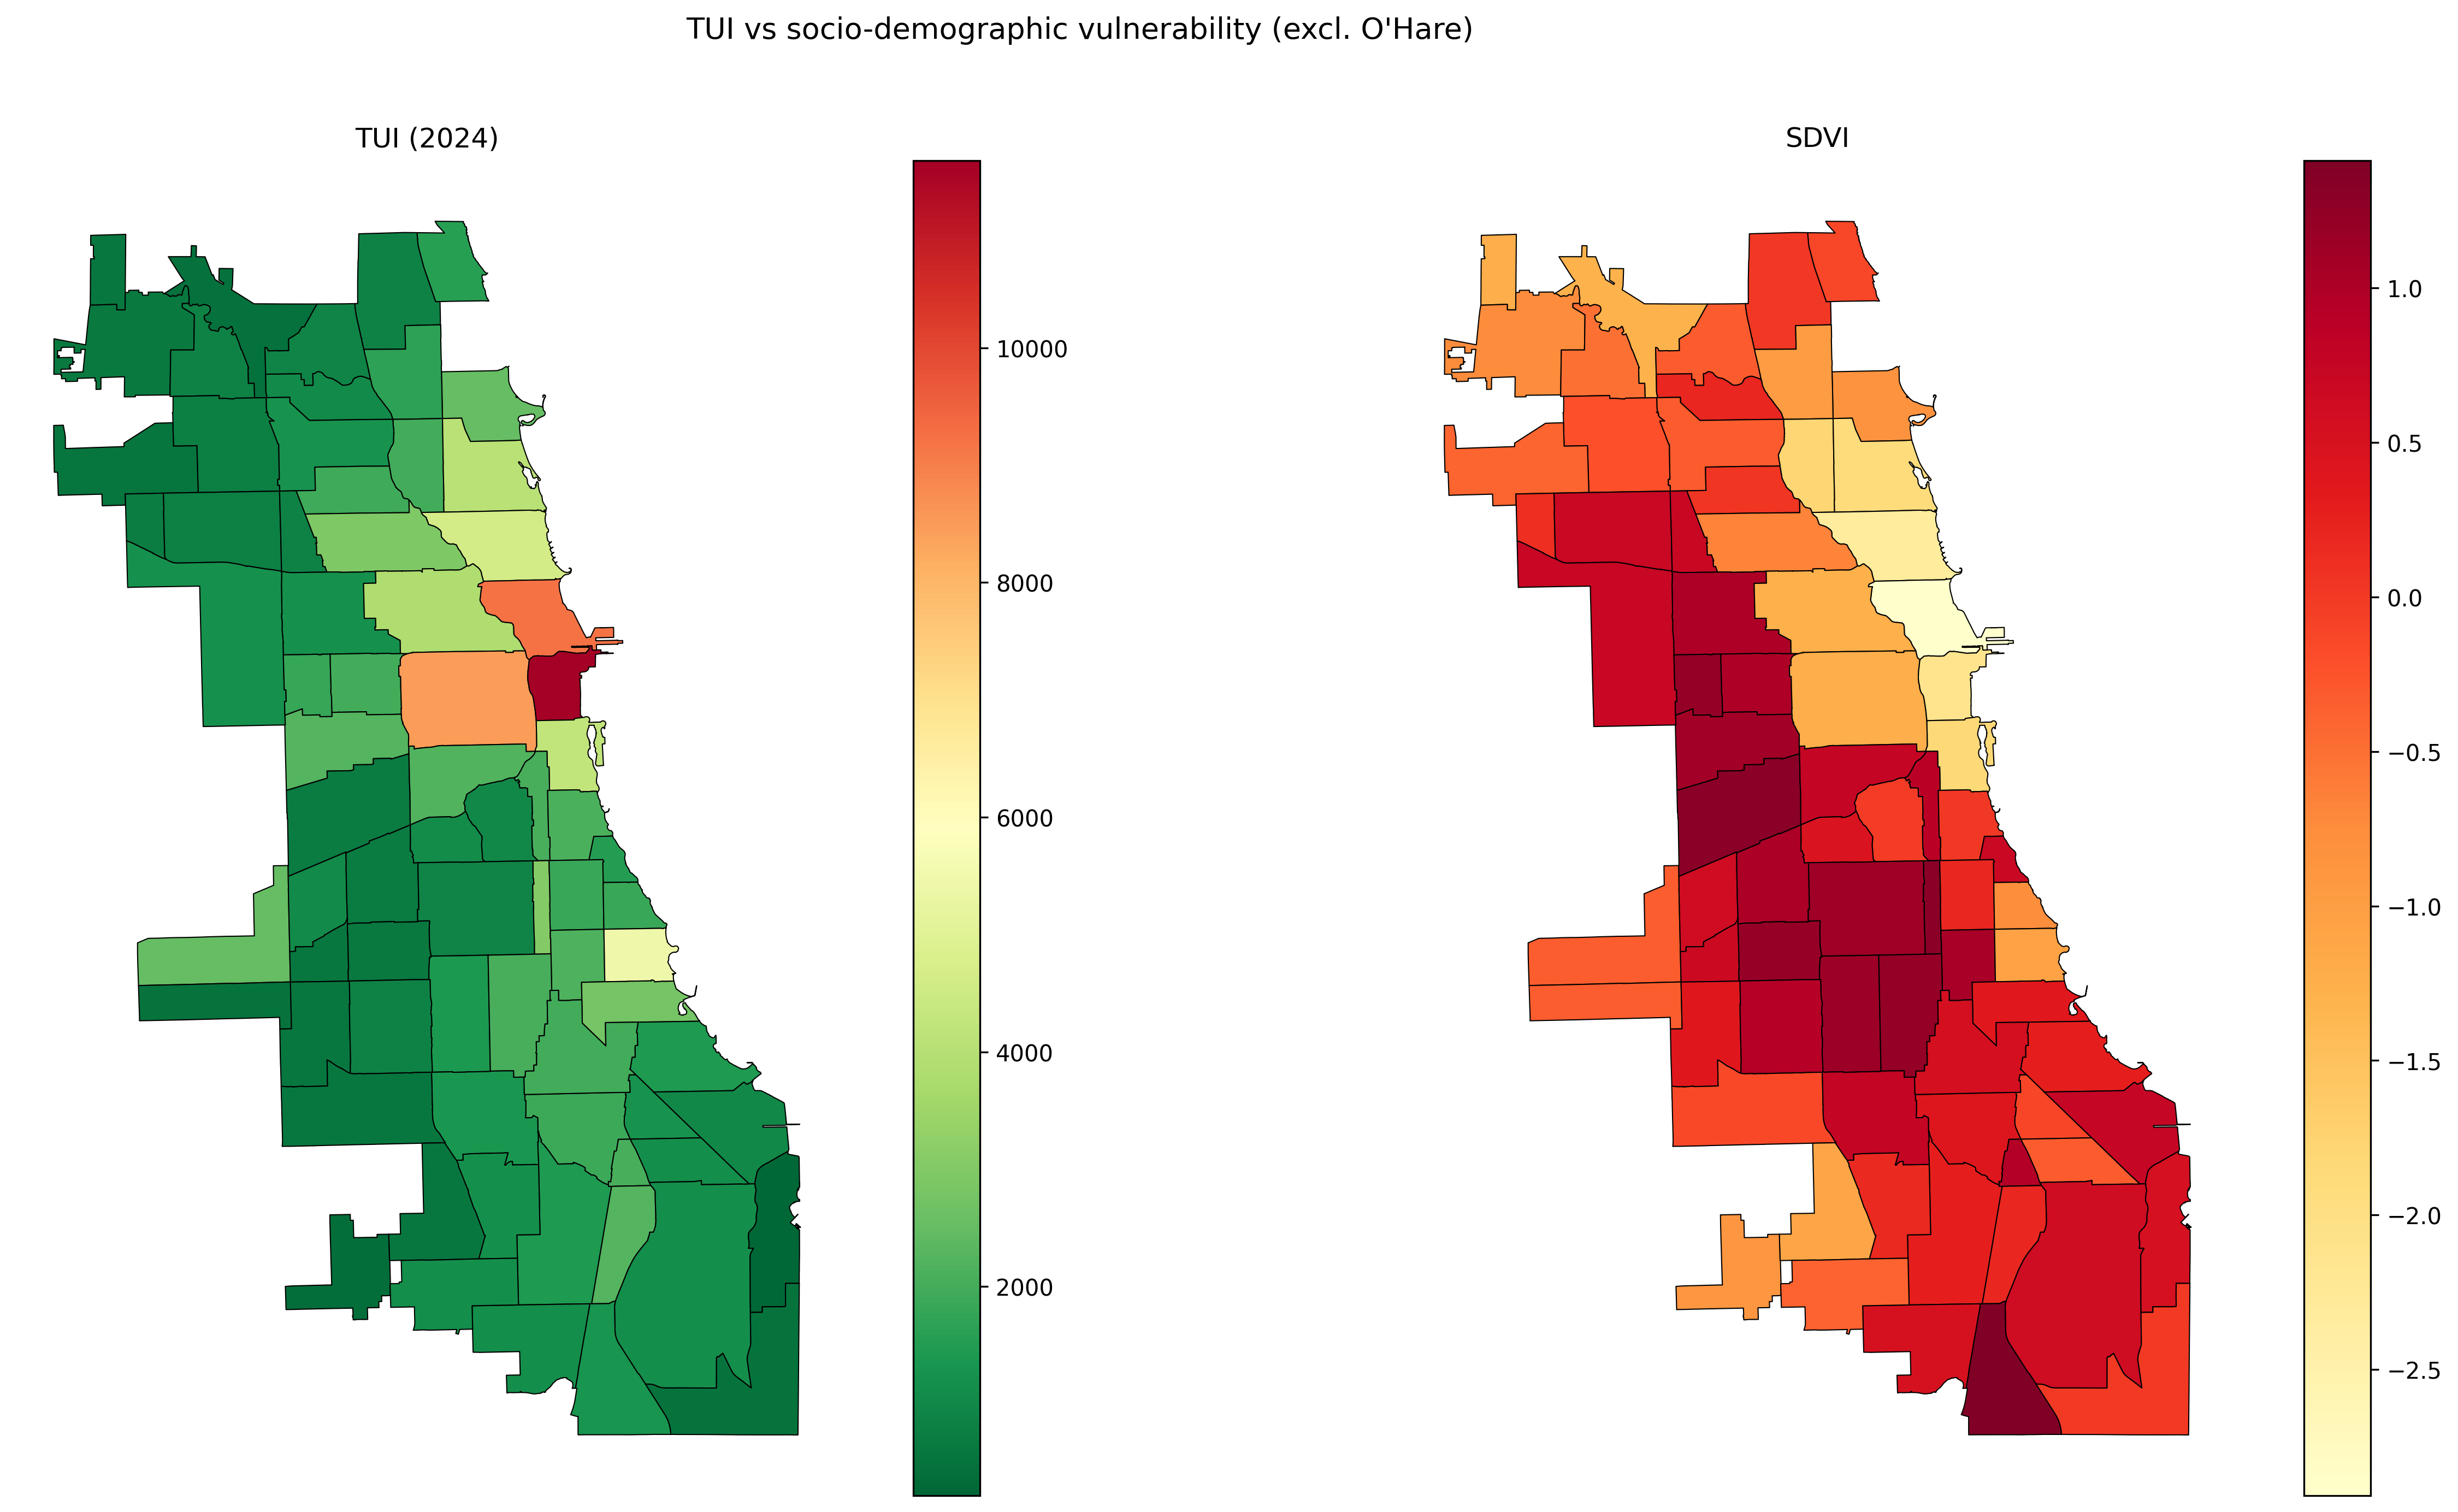
\includegraphics[width=0.95\textwidth]{figs/tui_sdvi_maps_2024.png}
    \caption{TUI and SDVI side by side, 2024 ($n=75$).}
    \label{fig:maps}
\end{figure}

\begin{figure}[htbp]
    \centering
    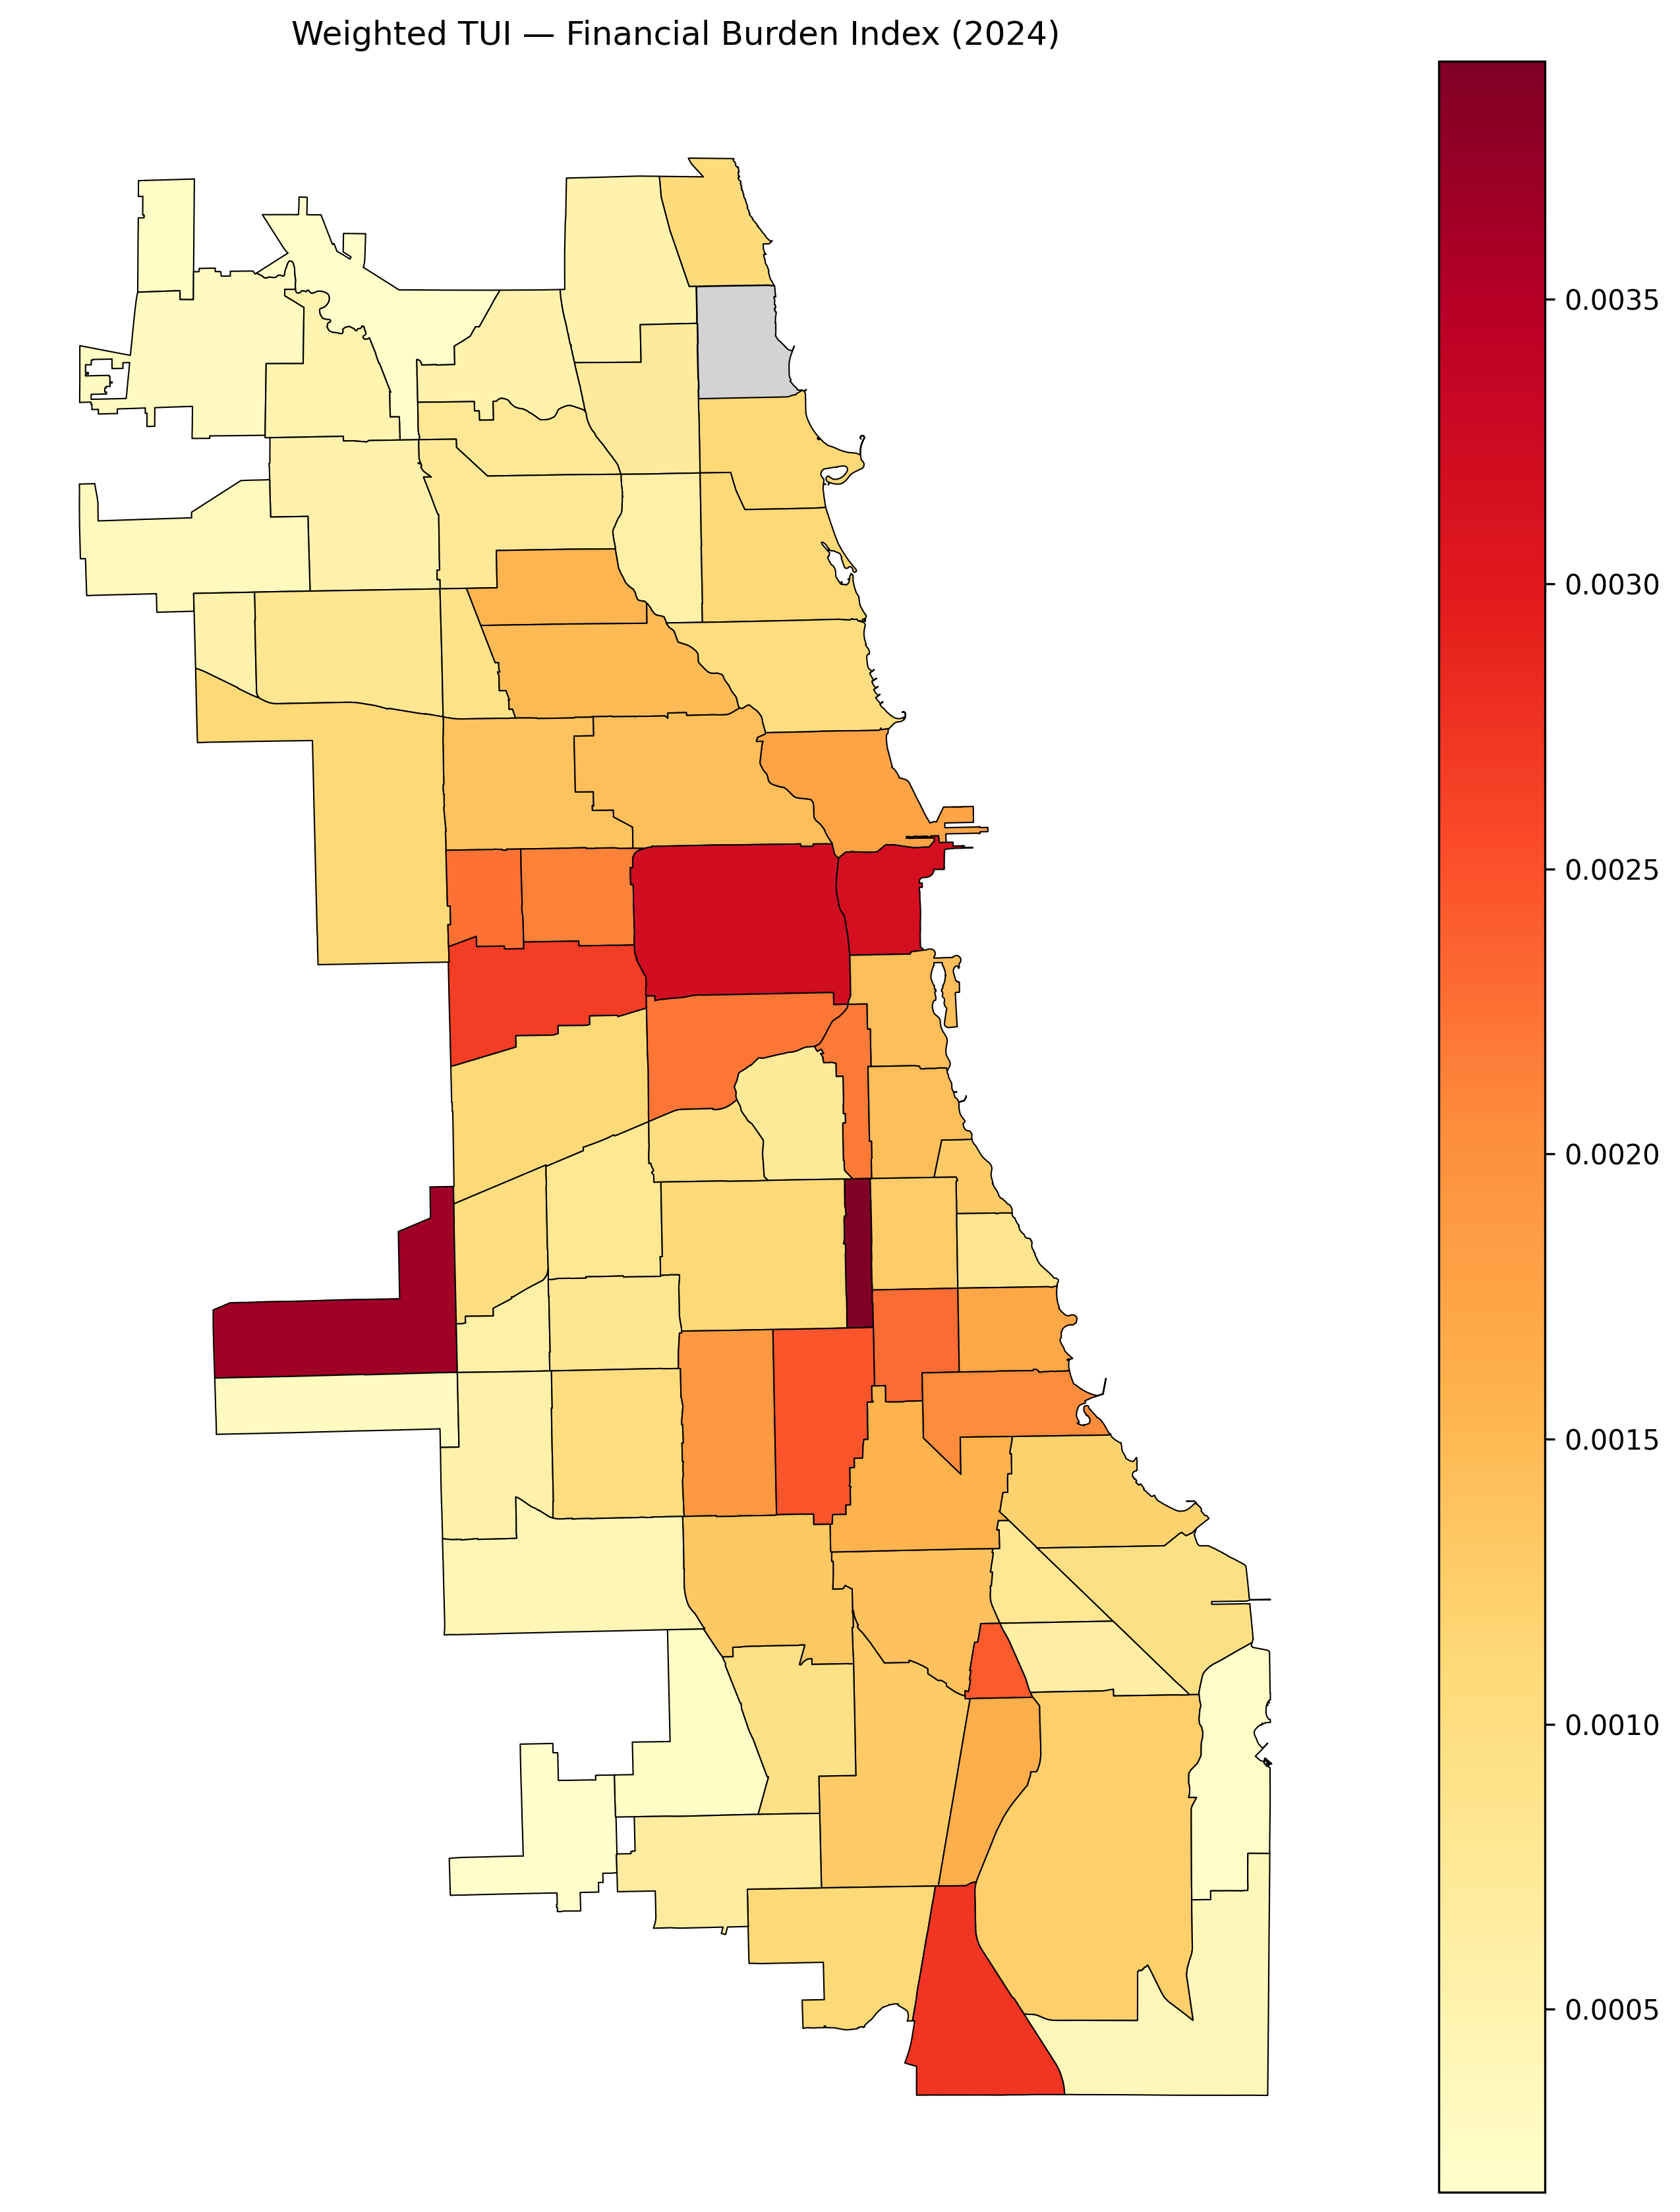
\includegraphics[width=0.48\textwidth]{figs/weighted_tui_2024.png}
    \caption{Weighted TUI (income-normalised financial burden), 2024.}
    \label{fig:wtui}
\end{figure}

\begin{figure}[htbp]
    \centering
    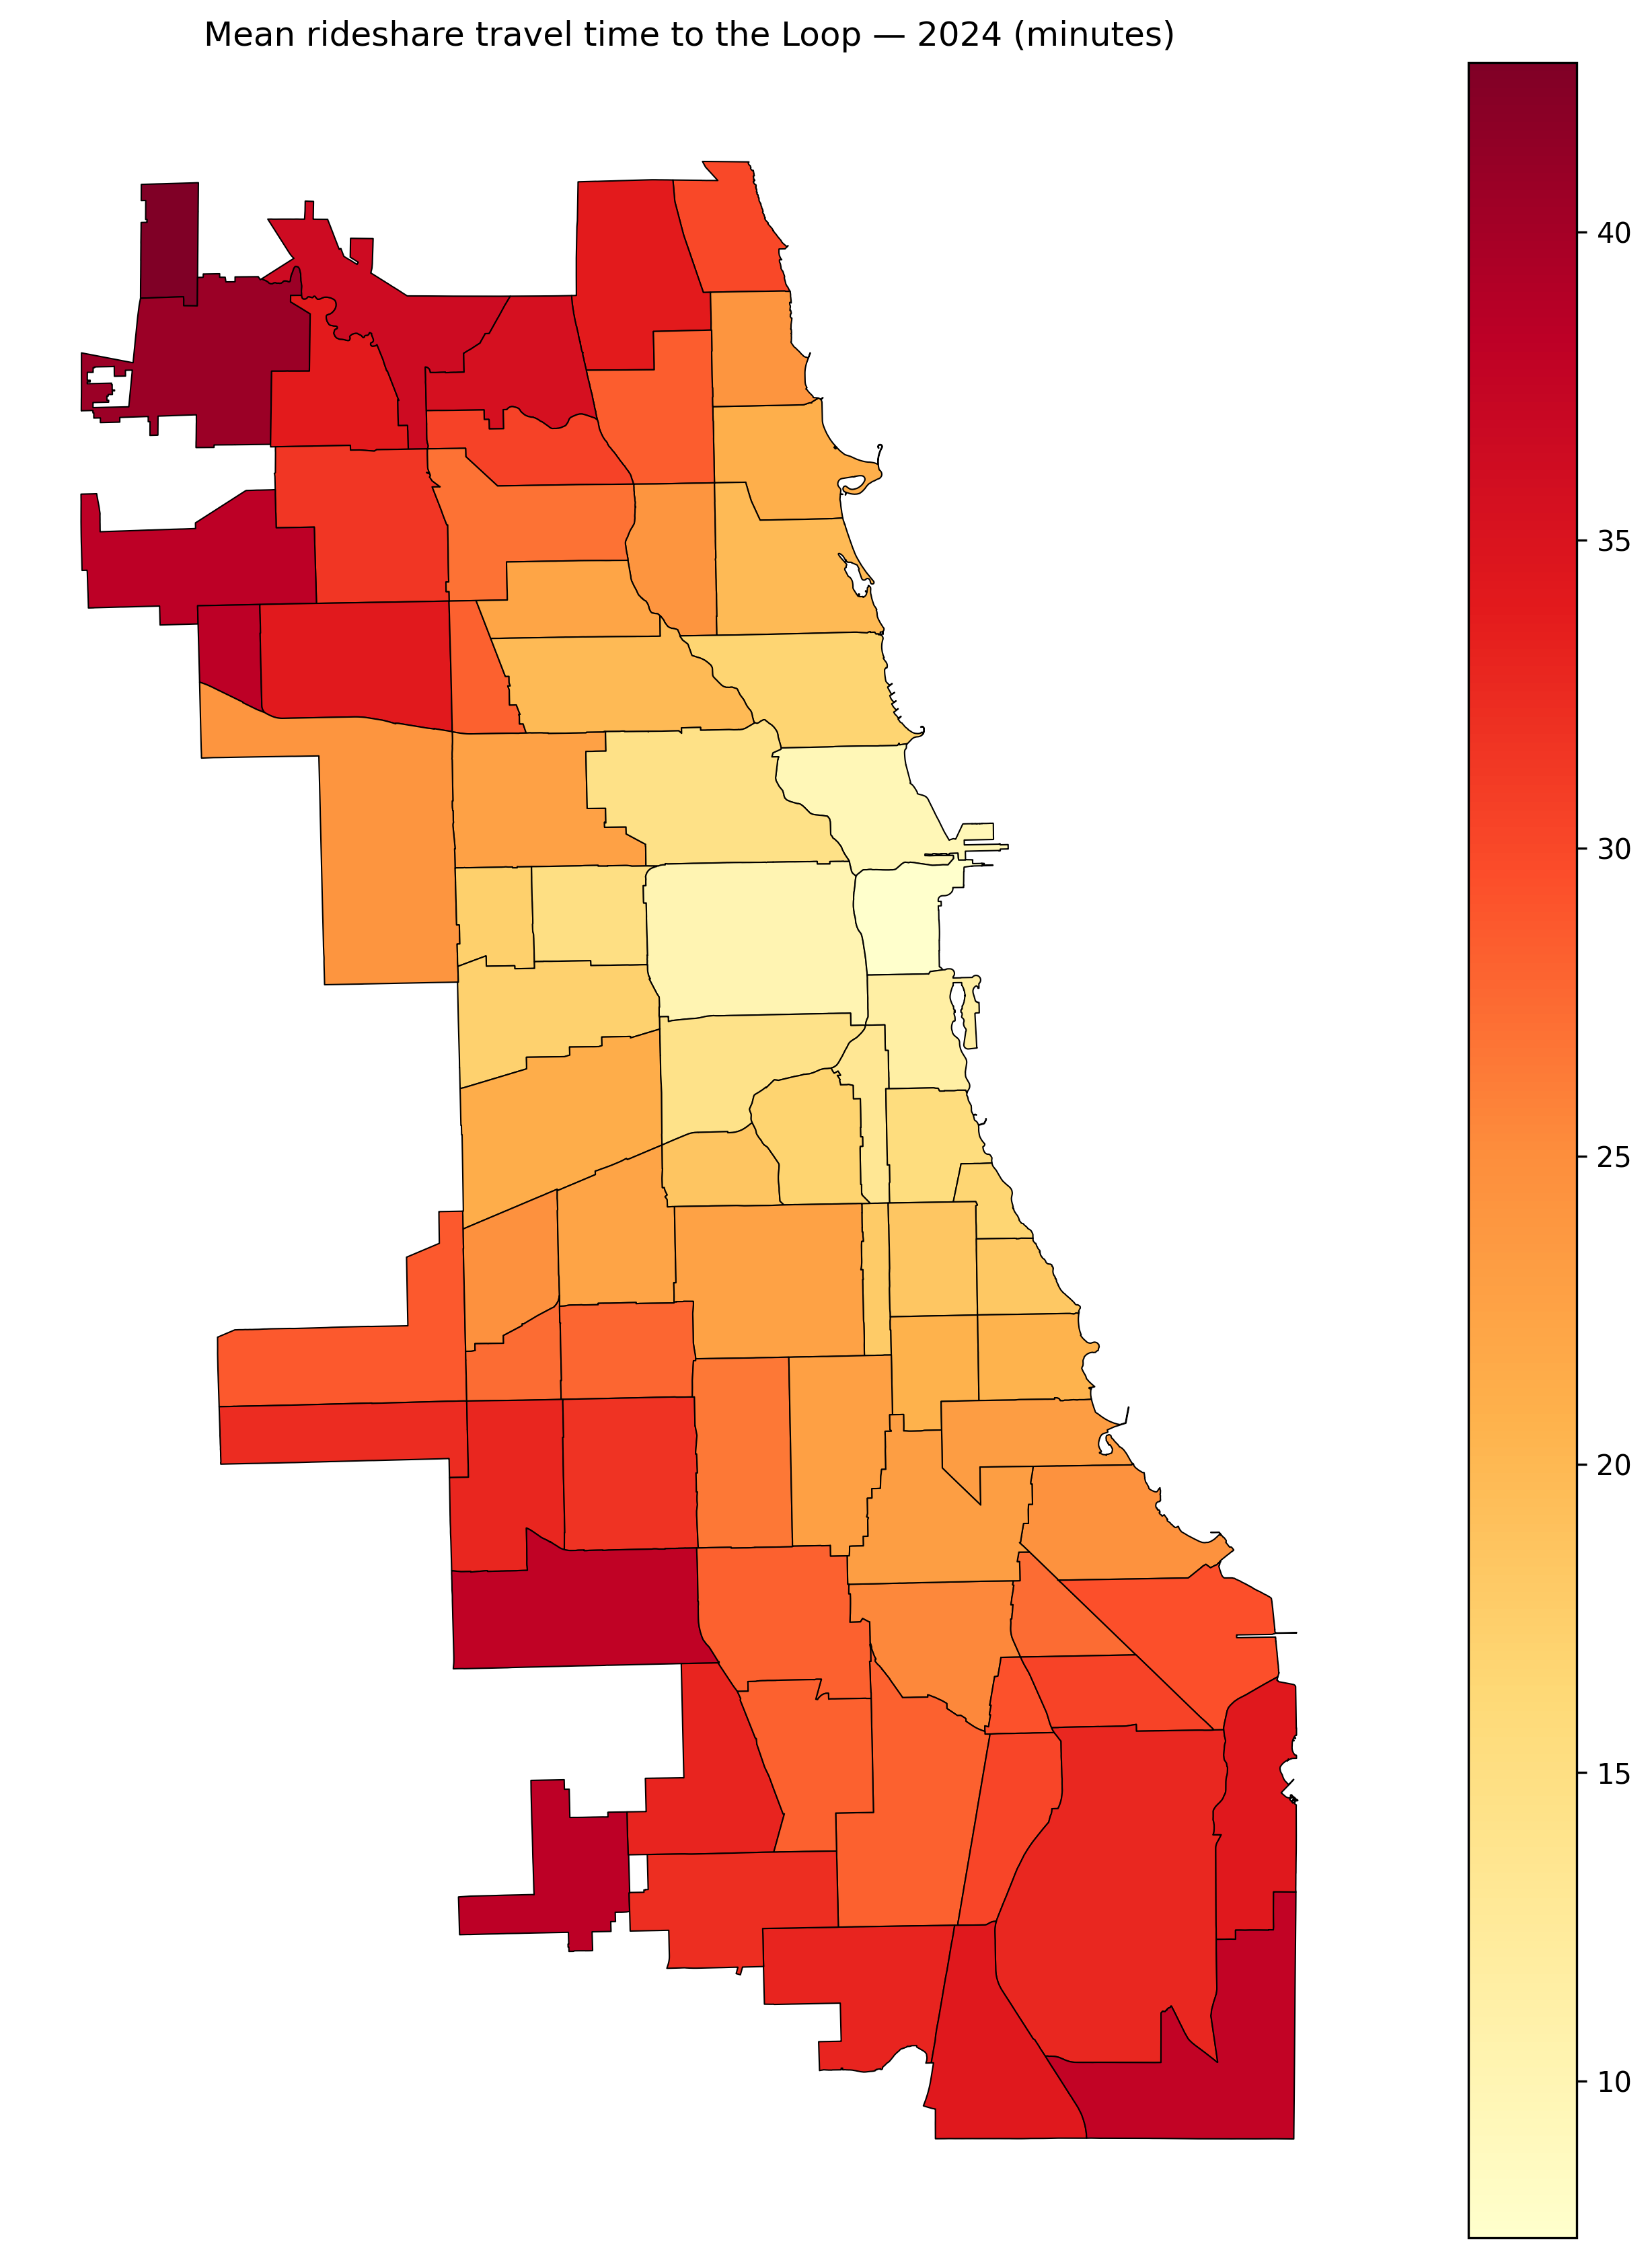
\includegraphics[width=0.48\textwidth]{figs/loop_travel_time_2024.png}
    \caption{Mean ridesourcing travel time to the Loop by pickup CA, 2024 (minutes).}
    \label{fig:loop}
\end{figure}

\begin{figure}[htbp]
    \centering
    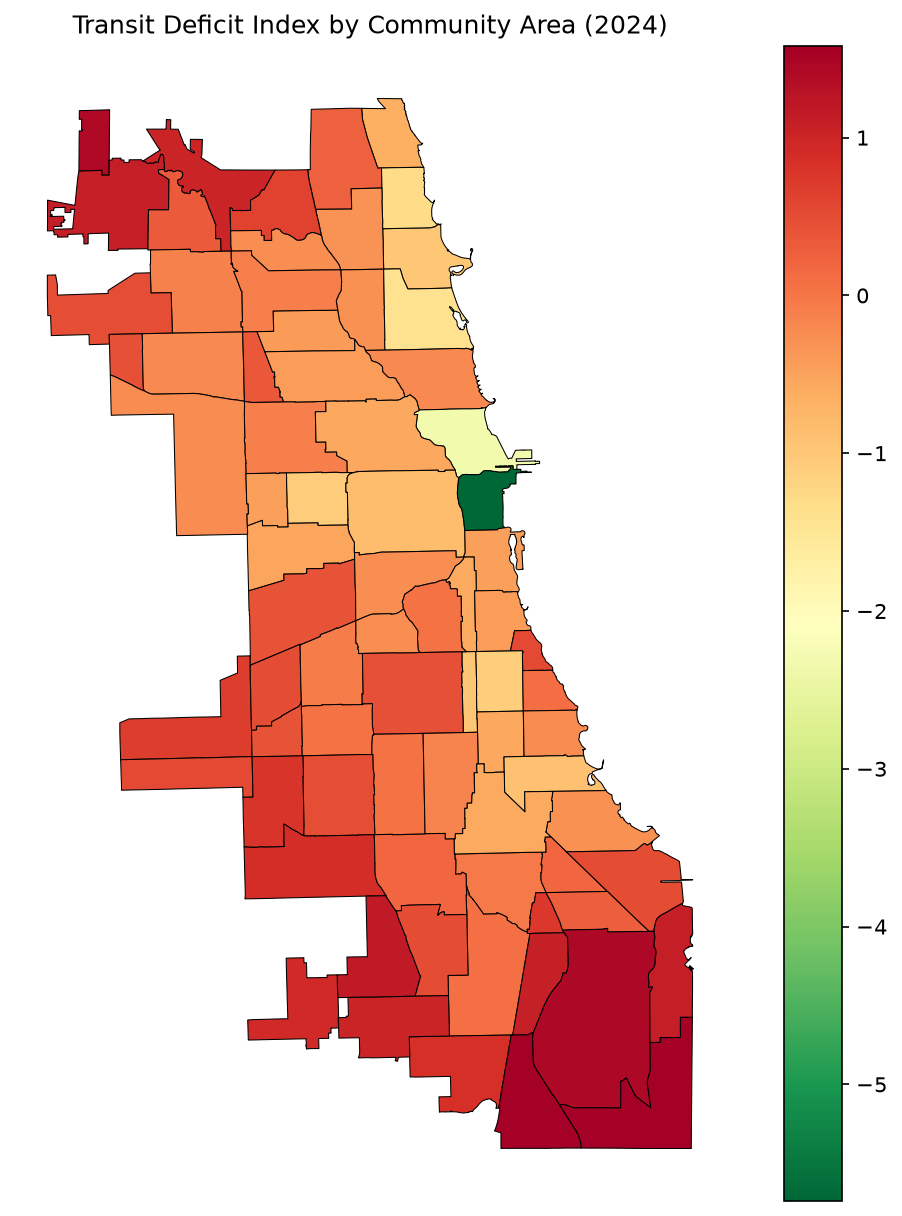
\includegraphics[width=0.48\textwidth]{figs/transit_deficit_2024.png}
    \caption{Transit Deficit Index by Community Area.}
    \label{fig:transit}
\end{figure}

\paragraph{Prediction model.}
The assignment does not require a forecasting model. Our design is cross-sectional for 2024 equity diagnosis. Monthly TNP series from 2018--2024 could nonetheless support ARIMA or panel models to project post-pandemic recovery trajectories by CA; we leave that extension to future work because the policy question here is spatial allocation in a single reference year, not trend extrapolation.

\paragraph{Classification or clustering model.}
No supervised classification task is specified. Exploratory spatial clustering is addressed through LISA on TUI rather than k-means on trip features. Vulnerability indices are deterministic composites (means of z-scores), not latent cluster labels. A possible extension would classify CAs into equity archetypes (high burden / low access, etc.) using decision trees on TUI, Weighted TUI, and transit deficit; we report those dimensions separately to keep interpretation transparent.

\paragraph{Optimization model.}
No optimisation model is required. The analysis is diagnostic and associational: we do not solve fleet repositioning, subsidy budget allocation, or integrated transit--TNP fare minimisation programmes. Such models would need demand elasticity parameters and budget constraints absent from open data; our maps and Table~\ref{tab:policy} instead prioritise zones for qualitative policy attention.

\newpage
\section{Conclusions}
This report tested whether ridesourcing in Chicago acts as a mobility equaliser in transit-poor, vulnerable peripheries, or as a complement concentrated where public transport and central activity are already strong. Across descriptive maps, correlation analysis, LISA clustering, and spatial regression on 75 Community Areas in 2024, the \textbf{compensatory hypothesis is rejected}.

\textit{Answer to the research question.} Ridesourcing does not primarily serve as an informal safety net in hardship peripheries. TUI peaks in the Loop, Near North Side, and Near West Side, correlates negatively with HSVI and SDVI ($r$ up to $-0.54$), and correlates positively with transit access ($r=0.75$). The Spatial Error Model confirms negative associations for HSVI and Loop travel time after accounting for spatial error ($\lambda=0.56$). Platforms reinforce existing urban cores rather than filling CTA gaps on the South and West Sides.

\textit{Usage versus burden.} Intensity and financial stress diverge. Weighted TUI elevates Fuller Park, Garfield Ridge, and Near West Side: residents who use TNP devote a larger income share than lakefront users despite lower pickup counts. Policy based on TUI heat maps alone would under-target burden hotspots and over-target visitor-driven central demand.

\textit{Spatial structure.} Moran's $I=0.61$ and LISA maps show statistically robust High--High clustering in the central corridor and Low--Low clustering across southwest and northwest residential zones. Garfield Ridge is the sole significant High--Low outlier, consistent with its high Weighted TUI. Very low-TUI far South areas (Riverdale, East Side) are visually extreme but not LISA-significant at $p<0.05$.

\textit{Peripherality.} Mean Loop travel time rises to 43 minutes from Edison Park; TUI falls with travel time ($r=-0.67$). Transit deficit and travel time correlate ($r=0.73$) yet travel time retains independent predictive power in regression. Spatial mismatch toward the Loop remains a structural constraint that ridesourcing does not resolve at the ecological scale.

\textit{Temporal stability.} The 2018 versus 2024 comparison (Section~\ref{sec:temporal}, Tables~\ref{tab:temporal_top}--\ref{tab:temporal_change}) shows Spearman $\rho=0.89$ across CAs: the core--periphery ranking is durable. Central absolute TUI fell sharply while some South Side zones grew from a low base, but 2024 levels still favour the lakefront and Loop.

\textit{Smart-city implication.} Digital mobility platforms should be integrated into multimodal planning as complements to public transit investment, not default substitutes. Priority zones for CTA frequency expansion (Riverdale, Hegewisch, South Deering) and means-tested subsidies (Fuller Park, Garfield Ridge) are identified in Table~\ref{tab:policy}. Richer open data on rider residence and accessibility would allow future work to separate dependency from visitor-driven intensity.

\subsection{Policy suggestions}
Findings imply cautious integration of TNP into smart-city mobility planning rather than treating platforms as automatic substitutes for CTA investment.

(1) \textit{Transit supply.} Expand bus and rail frequency in high-deficit peripheries (Riverdale, Hegewisch, South Deering, Edison Park) where Table~\ref{tab:policy} ranks deficit above $1.4$ standard deviations. Scheduled GTFS frequency should be part of capital planning metrics, not stop counts alone.

(2) \textit{Targeted subsidies.} Introduce means-tested ride vouchers or integrated transit--TNP passes where Weighted TUI is elevated (Fuller Park, Garfield Ridge, Near West Side). Subsidies should follow burden and access gaps, not central usage hotspots that already enjoy multimodal choice.

(3) \textit{Land use and job access.} Support policies that reduce dependence on long radial Loop trips \cite{kwan1998}: local employment centres, improved cross-town bus links, and equitable last-mile connections to rail. Ridesourcing cannot replace structural spatial mismatch.

(4) \textit{Data governance.} Advocate for richer open mobility fields (e.g.\ rider home CA where privacy permits, wheelchair-accessible vehicle availability) so future studies can separate resident dependency from visitor-driven intensity.

\begin{table}[htbp]
    \centering
    \caption{Priority Community Areas for transit investment and mobility subsidies (2024).}
    \label{tab:policy}
    \small
    \begin{tabular}{|l|l|r|l|r|}
        \hline
        \textbf{CA} & \textbf{High transit deficit} & \textbf{Deficit} & \textbf{High Weighted TUI} & \textbf{WTUI} \\
        \hline
        54 & Riverdale & 1.58 & Fuller Park (37) & 0.0039 \\
        55 & Hegewisch & 1.56 & Garfield Ridge (56) & 0.0037 \\
        51 & South Deering & 1.46 & Near West Side (28) & 0.0032 \\
        9  & Edison Park & 1.43 & Loop (32) & 0.0032 \\
        10 & Norwood Park & 1.10 & Riverdale (54) & 0.0027 \\
        \hline
    \end{tabular}
\end{table}

Low peripheral TUI must not be read as absence of demand. Subsidies should target burden and access gaps, not central usage hotspots. Appendix~A of the notebook confirms robustness of the main modelling choices.

\subsection{Limitations}\label{sec:limitations}
Several limitations bound interpretation of the results. We group them by data, measurement, methods, and scope.

\textit{Ecological inference and TUI definition.} All indicators are CA-level aggregates. Associations describe neighbourhood patterns, not individual riders (ecological fallacy). TUI measures pickup \emph{intensity} at origin, not resident \emph{dependency}: central CAs are inflated by commuters, tourists, and nightlife visitors because TNP records lack passenger home location. Low peripheral TUI must not be read as disinterest; it may reflect fare barriers and long travel times.

\textit{Temporal coverage and mismatch.} The main regression is cross-sectional for 2024. Monthly series exist for 2018--2019 and 2023--2024 only in our cache; 2020--2022 are missing locally, limiting pandemic-era panel analysis. Hardship and per capita income are from a 2008--2012 vintage while trips are from 2024. GTFS weekday schedules reflect the 2026 feed. We assume relative transit rankings and weekday frequency patterns are stable enough for cross-sectional comparison, but small temporal mismatches remain.

\textit{Multicollinearity among predictors.} HSVI, SDVI, and CCVI correlate at $r=0.86$--$0.96$; only HSVI enters regression. Transit deficit and mean Loop travel time correlate at $r=0.73$; both are retained because dropping travel time sharply worsens AIC, but SEM renders deficit non-significant. Variance inflation factors in Appendix~A remain below 5.

\textit{Spatial scale and exclusions.} Community Areas are coarse (77 zones). CA~76 (O'Hare) is excluded as a transport-hub outlier. LISA significance requires neighbour configuration; very low-TUI far South areas may be extreme descriptively without reaching $p<0.05$ locally.

\textit{Causal and policy limits.} Findings are associational. Platform pricing, driver supply, CTA service cuts, and land-use change are not modelled as causal drivers. Weighted TUI uses median fares, not trip-weighted mean fares or tip data. We do not observe wheelchair-accessible vehicle availability or wait times.

\textit{Robustness.} Appendix~A of the notebook confirms stable coefficient signs under reduced specifications and VIF diagnostics. Reduced spatial models worsen AIC and can flip SEM versus SLAG preference, reinforcing retention of the full model for the main conclusions.

\newpage
\addcontentsline{toc}{section}{References}
\section*{References}
\bibliographystyle{IEEEtran}
\bibliography{references.bib}

\newpage
\appendix
\section{AI Usage}
Generative AI (Cursor) was used in a supporting role during this project: code review and consistency checks on \texttt{SmartCities\_RideSharing.ipynb} and \texttt{utils.py}; cross-checking numerical results quoted in this report against notebook outputs; drafting and refining the English text of the essay; and assistance with Git versioning (commits, conflict resolution, and repository hygiene). Analysis design, indicator definitions, modelling choices, and interpretation remain the authors' responsibility.

\end{document}
